\documentclass[]{article}
\usepackage{lmodern}
\usepackage{amssymb,amsmath}
\usepackage{ifxetex,ifluatex}
\usepackage{fixltx2e} % provides \textsubscript
\ifnum 0\ifxetex 1\fi\ifluatex 1\fi=0 % if pdftex
  \usepackage[T1]{fontenc}
  \usepackage[utf8]{inputenc}
\else % if luatex or xelatex
  \ifxetex
    \usepackage{mathspec}
  \else
    \usepackage{fontspec}
  \fi
  \defaultfontfeatures{Ligatures=TeX,Scale=MatchLowercase}
\fi
% use upquote if available, for straight quotes in verbatim environments
\IfFileExists{upquote.sty}{\usepackage{upquote}}{}
% use microtype if available
\IfFileExists{microtype.sty}{%
\usepackage{microtype}
\UseMicrotypeSet[protrusion]{basicmath} % disable protrusion for tt fonts
}{}
\usepackage[margin=1in]{geometry}
\usepackage{hyperref}
\hypersetup{unicode=true,
            pdftitle={Método},
            pdfauthor={Said E. Jiménez},
            pdfborder={0 0 0},
            breaklinks=true}
\urlstyle{same}  % don't use monospace font for urls
\usepackage{longtable,booktabs}
\usepackage{graphicx,grffile}
\makeatletter
\def\maxwidth{\ifdim\Gin@nat@width>\linewidth\linewidth\else\Gin@nat@width\fi}
\def\maxheight{\ifdim\Gin@nat@height>\textheight\textheight\else\Gin@nat@height\fi}
\makeatother
% Scale images if necessary, so that they will not overflow the page
% margins by default, and it is still possible to overwrite the defaults
% using explicit options in \includegraphics[width, height, ...]{}
\setkeys{Gin}{width=\maxwidth,height=\maxheight,keepaspectratio}
\IfFileExists{parskip.sty}{%
\usepackage{parskip}
}{% else
\setlength{\parindent}{0pt}
\setlength{\parskip}{6pt plus 2pt minus 1pt}
}
\setlength{\emergencystretch}{3em}  % prevent overfull lines
\providecommand{\tightlist}{%
  \setlength{\itemsep}{0pt}\setlength{\parskip}{0pt}}
\setcounter{secnumdepth}{0}
% Redefines (sub)paragraphs to behave more like sections
\ifx\paragraph\undefined\else
\let\oldparagraph\paragraph
\renewcommand{\paragraph}[1]{\oldparagraph{#1}\mbox{}}
\fi
\ifx\subparagraph\undefined\else
\let\oldsubparagraph\subparagraph
\renewcommand{\subparagraph}[1]{\oldsubparagraph{#1}\mbox{}}
\fi

%%% Use protect on footnotes to avoid problems with footnotes in titles
\let\rmarkdownfootnote\footnote%
\def\footnote{\protect\rmarkdownfootnote}

%%% Change title format to be more compact
\usepackage{titling}

% Create subtitle command for use in maketitle
\newcommand{\subtitle}[1]{
  \posttitle{
    \begin{center}\large#1\end{center}
    }
}

\setlength{\droptitle}{-2em}

  \title{Método}
    \pretitle{\vspace{\droptitle}\centering\huge}
  \posttitle{\par}
    \author{Said E. Jiménez}
    \preauthor{\centering\large\emph}
  \postauthor{\par}
      \predate{\centering\large\emph}
  \postdate{\par}
    \date{6 de marzo de 2019}


\begin{document}
\maketitle

{
\setcounter{tocdepth}{3}
\tableofcontents
}
\subsection{Participantes}\label{participantes}

Se incluyeron 20 personas voluntarias (18 mujeres), en un rango de edad
de 19-33 años, su nivel educativo mínimo fue licenciatura, su ocupación
principal fue estudiantes y eran solteros. Todos los participantes
reportaron no tener historial médico de tipo neurológico ni psiquiátrico
al momento del experimento. Los participantes acudieron al estudio con
un amigo considerado \emph{cercano} por ellos mismos, quien cumplía las
siguientes características: era una persona del mismo sexo que el
participante, no tenía un vínculo familiar y no se trataba de una
persona con una relación de tipo sentimental y/o sexual.

\subsection{Materiales y
Procedimiento}\label{materiales-y-procedimiento}

Todos los participantes realizaron una adaptación de la tarea de
confianza y promesas presentada por Baumgartner (2009), que consiste en
24 ensayos entre dos jugadores \textbf{A} y \textbf{B}, el jugador
\textbf{A} tiene originalmente 0 pesos mexicanos y el jugador \textbf{B}
tiene 2 pesos, al jugador \textbf{B} se le presenta la oportunidad de
invertir su dinero al jugador \textbf{A} o conservarlo, si invierte su
dinero se multiplica por 5 pesos, de modo que el jugador \textbf{A}
recibe 10 pesos. Finalmente, el jugador \textbf{A} toma la decisión de
pagar la mitad al jugador \textbf{B} o quedarse los 10 pesos. La
estructura descrita se repite en 24 ensayos, sin embargo, en 4 de los
ensayos el jugador \textbf{A} puede enviar una promesa a \textbf{B}, las
promesas son que \emph{siempre}, \emph{casi siempre}, \emph{algunas
veces} o \emph{nunca} pagaran la mitad. Cada promesa es válida por tres
ensayos, de modo que 12 de los ensayos tienen el efecto de la promesa y
los otros 12 no lo tienen.

La variación respecto a la tarea original es que en nuestro experimento
se presentaron tres compañeros de juego con tres niveles de cercanía
social en el papel del jugador \textbf{B}: \textbf{computadora}
(cercanía nula), \textbf{confederado} (cercanía baja) y \textbf{amigo}
(cercanía alta), mientras que el participante principal siempre fungió
el papel del jugador \textbf{A}. Cada compañero de juego realizó el rol
de \textbf{B} en 8 de los 24 ensayos totales, sin embargo, tanto la
condición de promesas como la de cercanía social fueron presentadas al
sujeto \textbf{A} en orden pseudoaleatorio, lo que significa que se
realizó la aleatorización de los ensayos una vez y se mantuvo el mismo
orden para todos los sujetos. Con el fin de simplificar la tarea y
homogeneizar la experiencia de todos nuestros participantes, se
programaron \emph{a priori} las decisiones de los compañeros \textbf{B}
sobre si invertían o no su monto inicial, se programó que los tres
compañeros decidieran invertir en 6 ensayos y no invertir en 2, los
cuales también se presentaron al sujeto \textbf{A} en orden
pseudoaleatorio. La historia encubierta para todos nuestros sujetos en
el papel de \textbf{A} fue que estarían jugando en tiempo real con su
amigo, el confederado (que se le dijo que sería otra persona desconocida
de su mismo sexo) y la computadora.

En la figura 1 se muestra un diagrama de la cronología de la tarea
experimental con las duraciones de cada fase en segundos, cada caja de
izquierda a derecha representa una pantalla que se le mostró a los
sujetos de manera secuencial. La parte A\(_{1}\) corresponde a un
ejemplo de los ensayos sin promesas y la A\(_{2}\) de los ensayos con
promesas. La fase de fijación sólo consistió en un período en el que el
sujeto prestaba atención sin realizar ninguna conducta en particular, la
\textbf{fase de promesas} en la parte A\(_{1}\) le indicó al sujeto que
los siguientes tres ensayos se podían decidir sin el efecto de la
promesa, mientras que en A\(_{2}\) se le pidió al sujeto que decidiera
entre \emph{siempre}, \emph{casi siempre}, \emph{algunas veces} o
\emph{nunca} pagar la mitad. A lo anterior, le siguió otro período de
fijación, posteriormente los ensayos tanto en A\(_{1}\) como en
A\(_{2}\) continuaron aproximadamente de la misma forma, en la
\textbf{fase de anticipación/asignación} se le indicó a los sujetos
quién era su compañero de juego para ese ensayo (computadora,
confederado o amigo) y se le dió el mensaje de que su compañero estaba
tomando su decisión, posteriormente en la \textbf{fase de decisión} se
le dió al participante la información sobre cuál había sido la decisión
de su compañero (si invirtió sus 2 pesos o no), se le recordaba su nivel
de promesas (si se trataba de ensayos con promesas) y, en el caso de que
su compañero hubiera invertido, se le pedía que decidiera si pagaba de
regreso o no. Finalmente, en la \textbf{fase de feedback} se mostraban
los pagos para ese ensayo y se repetía la secuencia. La tarea se
programó en PsychoPy2 versión 1.84.2, que registraba las respuestas de
los sujetos y los tiempos de reacción en segundos.

\begin{figure}

{\centering 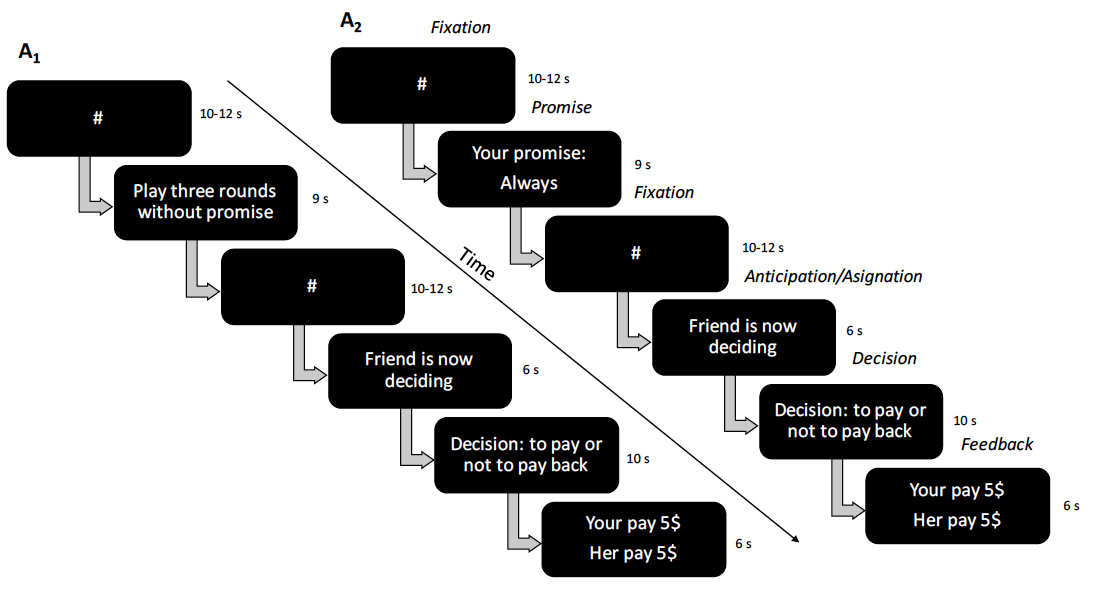
\includegraphics[width=0.8\linewidth]{/Users/saidjimenez/Documents/R/github_Said/social_closeness/Manuscript/figures/task} 

}

\caption{Task of promises and social closeness}\label{fig:figA}
\end{figure}

\subsection{Modelamiento Bayesiano}\label{modelamiento-bayesiano}

\subsubsection{Análisis descriptivo}\label{analisis-descriptivo}

Se obtuvieron las proporciones de las decisiones pagar o no pagar la
mitad, así como las promesas realizadas, posteriormente se calcularon
las variaciones en las proporciones de acuerdo a los compañeros de juego
y la condición de presencia o ausencia de promesas.

\subsubsection{Modelo Jerárquico}\label{modelo-jerarquico}

Se utilizó inferencia bayesiana para evaluar el efecto de las
condiciones experimentales en la tasa de pago a nivel individual y
poblacional. Para tal propósito se realizó un modelo jerárquico que
asume que la incertidumbre en el efecto de promesas y parejas sobre la
conducta de cada individuo proviene de distribuciones poblacionales
comunes para los parámetros del modelo:

\[
\begin{aligned}
&y_i \sim \mathrm{Bernoulli}(\theta_i) \\
&\mathrm{logit(\theta_i)} = \mathbf{X}\beta  +  \mathbf{Z}u
\end{aligned}
\] En el modelo anterior, cada decisión \(y_i\) proviene de una
distribución Bernoulli con probabilidad de pagar \(\theta_i\), el
objetivo del modelo jerárquico es predecir cada decisión a través la
combinación lineal de los predictores transformados por su función
ligadora inversa \(\mathrm{logit}\). En el modelo anterior, \(\beta\) y
\(u\) son coeficientes a nivel poblacional y nivel individual
respectivamente, mientras que \(\mathbf{X}\), \(\mathbf{Z}\) son sus
correpondientes matrices del diseño.

El modelo estima que la probabilidad \(\theta_i\) de que en cada ensayo
se decida pagar la mitad está en función del efecto de la presencia de
promesas \(\beta^{promise}\), así como de los compañeros con cercanía
social baja \(\beta^{confederate}\) y alta \(\beta^{friend}\). También
asume que pueden existir diferencias individuales en el desempeño
durante la tarea, las cuales son captadas por los parámetros \(u\) y
constituyen ajustes a los coeficientes poblacionales. Cabe remarcar que
el modelo evalúa explícitamente la incertidumbre respecto a \(u\), lo
cual es una ventaja con relación a los modelos que asumen que \(u\) es
parte del término de error.

El modelo se programó en R por medio del paquete \textbf{brms}, que
realiza la inferencia mediante el muestreo por Markov chain Monte Carlo
a través de \textbf{Stan}. Las distribuciones posteriores de todos los
parámetros fueron aproximadas con cuatro cadenas de 2000 iteraciones
cada una, las primeras 1000 iteraciones de cada cadena fueron
descartadas (periodo de calentamiento), para un total de 4000 muestras
post-calentamiento. La convergencia del modelo fue evaluada a través de
la inspección visual de las cadenas y el cálculo del estadístico
\(\hat{R}\), que para todos los parámetros fue de 1, lo que se
interpreta como convergencia.

\subsubsection{Modelamiento de mezclas
latentes}\label{modelamiento-de-mezclas-latentes}

Asume que las decisiones de los individuos podrían provenir de una
combinación (o \emph{mezcla}) de procesos psicológicos no observables
(\emph{latentes}), el rasgo latente más importante en este experimento
es la (des)honestidad. Se modelaron las diferencias en las tasas de pago
entre participantes como una combinación de \(N\) distribuciones de
subpoblaciones. El modelo asumió que las tasas de pago provenían de una
o dos mezclas de distribuciones, o grupos latentes.

El modelo de una mezcla, asumía que cada decisión \(d_{i,j}\) de cada
sujeto provenía de una distribución Bernoulli con probabilidad
\(\theta_{i,j}\). Asimismo que \(\theta_{i,j}\) provenía de una
distribución jerárquica Beta con parámetros \(\alpha\) y \(\beta\). La
distribución Beta fue reparametrizada en términos de media \(\mu\) y
precisión \(\lambda\), ya que \(\mu = \alpha/(\alpha + \beta)\) y
\(\lambda = \alpha + \beta\).

\[
\begin{aligned}
&\mu \sim \mathrm{Uniform}(0, 1)\\
&\lambda \sim \mathrm{Uniform}(4, 100)\\
&\theta_{i,j} \sim \mathrm{Beta}(\mu\lambda, (1 - \mu)\lambda)\\
&d_{i,j} \sim \mathrm{Bernoulli}(\theta_{i,j}) 
\end{aligned}
\]

El modelo de dos mezclas es aproximadamente igual al anterior, sin
embargo ahora asume que las decisiones provienen de una \emph{mezcla} de
las distribuciones de dos subpoblaciones, una distribución Beta con
parámetros \(\mu_1\lambda_1\) y \((1 - \mu_1) \lambda_1\) y otra con
párametros \(\mu_2\lambda_2\) y \((1 - \mu_2) \lambda_2\), el parámetro
\(z_i\) determina la probabilidad de que cada sujeto pertenezca a uno de
dos grupos latentes, se distribuye Bernoulli con probabilidad \(\phi\),
que a su vez sigue una distribución inicial Beta relativamente poco
informativa.

Se presenta el modelo de 2 mezclas con la notación propuesta por Lee,
nodos cuadrados representan variables discretas y nodos circulares
variables numéricas. Los nodos sombreados representan variables
observadas, mientras que los nodos no sombreados son variables latentes.
Los dos rectángulos representan repeticiones de la relación entre los
parámetros del modelo para cada sujeto \(i\) y ensayo \(j\). Se
determinó que un individuo pertenecía al grupo de \emph{Deshonestos} si
\(z_i < 0.5\), dado que la probabilidad de que ese sujeto pagara la
mitad en cada ensayo es baja, mientras que se consideró que un individuo
pertenecía al grupo de \emph{Honestos} si \(z_i > 0.5\), dado que la
probabilidad de que el individuo pague la mitad en cada ensayo es alta.

\[
\begin{aligned} 
&\mu_1 \sim \mathrm{Uniform}(0, 1)\\
&\mu_2 \sim \mathrm{Uniform}(\mu_1, 1)\\
&\lambda_{1:2} \sim \mathrm{Uniform}(4, 100)\\
&z_i \sim \mathrm{Bernoulli}(\phi)\\
&\theta_{i,j} \sim \Bigg\{
  \begin{array} {lr} 
    \mathrm{Beta}(\mu_1\lambda_1, (1 - \mu_1)\lambda_1) \quad \mbox{if} \quad z_i = 0 \\
    \mathrm{Beta}(\mu_2\lambda_2, (1 - \mu_2)\lambda_2) \quad \mbox{if} \quad z_i = 1
  \end{array} \\
&d_{i,j} \sim \mathrm{Bernoulli}(\theta_{i,j})\\
&\phi \sim \mathrm{Beta}(5, 5)
\end{aligned}
\]

Los modelos de 1 y 2 mezclas, se programaron en R mediante el paquete
\textbf{rjags}, que realiza la inferencia mediante el muestreo por
Markov chain Monte Carlo a través de \textbf{JAGS}. Las distribuciones
posteriores de todos los parámetros fueron aproximadas con tres cadenas
de 26000 iteraciones cada una, se descartaron las primeras 6000 de cada
cadena como periodo de calentamiento, para un total de 60000 muestras
post-calentamiento. La convergencia del modelo fue evaluada a través de
la inspección visual de las cadenas y el cálculo del estadístico
\(\hat{R}\), que varió de 1 a 1.05 para todos los parámetros lo que
indica convergencia.

\subsubsection{Modelamiento de los tiempos de
reacción}\label{modelamiento-de-los-tiempos-de-reaccion}

Un hallazgo constante en la investigación sobre engaño y deshonestidad,
es la diferencia en los tiempos de reacción entre quienes toman
decisiones \emph{deshonestas} vs.~decisiones \emph{honestas}, en
general, se han encontrado latencias breves en personas
\emph{deshonestas} en comparación con las de las personas
\emph{honestas}.

Se estimaron las medias poblacionales del grupo de deshonestos y
honestos mediante un modelo bayesiano jerárquico que asumía que el
tiempo de reacción proviene de una distribución
\(rt_i \sim \mathrm{Half-Normal}(0, 5)\) (dado que no puede haber
tiempos de reacción negativos), con parámetros \(\mu_{Dishonest}\) y
\(\mu_{Honest}\) y desviación estándar común \(\sigma\).

Asimismo, se modeló la variabilidad intrasujeto en los tiempos de
reacción por medio de interceptos variantes por participante. El modelo
se ajustó en R por medio de \textbf{brms} y \textbf{Stan} en condiciones
iguales a las descritas anteriormente para el modelo jerárquico y obtuvo
resultados adecuados de convergencia para todos los parámetros,
\(\hat{R} = 1\).

\subsubsection{Contraste de hipótesis}\label{contraste-de-hipotesis}

Para los modelos de la tasa de pago y tiempo de reacción se utilizó el
factor de Bayes por medio del método de Savage-Dickey, que calcula la
razón de la densidad de la distribución posterior sobre la densidad de
la distribución inicial de algún parámetro en el punto de interés.
Específicamente para el modelo de la tasa de pago, se evaluó la
hipótesis de si las promesas tendrían un efecto positivo en las tasas de
pago (\(H_1: \beta^{promise} > 0\)), así como si la cercanía social alta
(amigo) tendría mayores tasas de pago que la cercanía social baja
(confederado) (\(H_1: \beta^{friend} - \beta^{confederate} > 0\)). Para
el modelo del tiempo de reacción, la hipótesis fue si los
\emph{deshonestos} tendrían tiempos breves en comparación con los
\emph{honestos} (\(H_1: \mu_{Dishonest} - \mu_{Honest} < 0\)).

\subsubsection{Comparación de modelos}\label{comparacion-de-modelos}

Los modelos de una y dos mezclas se compararon por medio del criterio de
información DIC (deviance information criteria), en el que los puntajes
bajos indican mejores modelos. La estimación de la diferencia entre el
modelo de 1 y 2 mezclas favorece al modelo de dos mezclas
(\(\mathrm{Difference}= 1.21\), \(\mathrm{SE}= 3.49\)).

\subsection{Resultados}\label{resultados}

\subsubsection{Descriptivos}\label{descriptivos}

Se muestra en la figura 2, la frecuencia de veces en que los
participantes pagaron la mitad, así como la frecuencia de promesas que
fueron seleccionadas. En la figura 3, se muestra la proporción de pagos
realizados dependiendo de cada pareja y de la condición de promesas.

\begin{figure}

{\centering 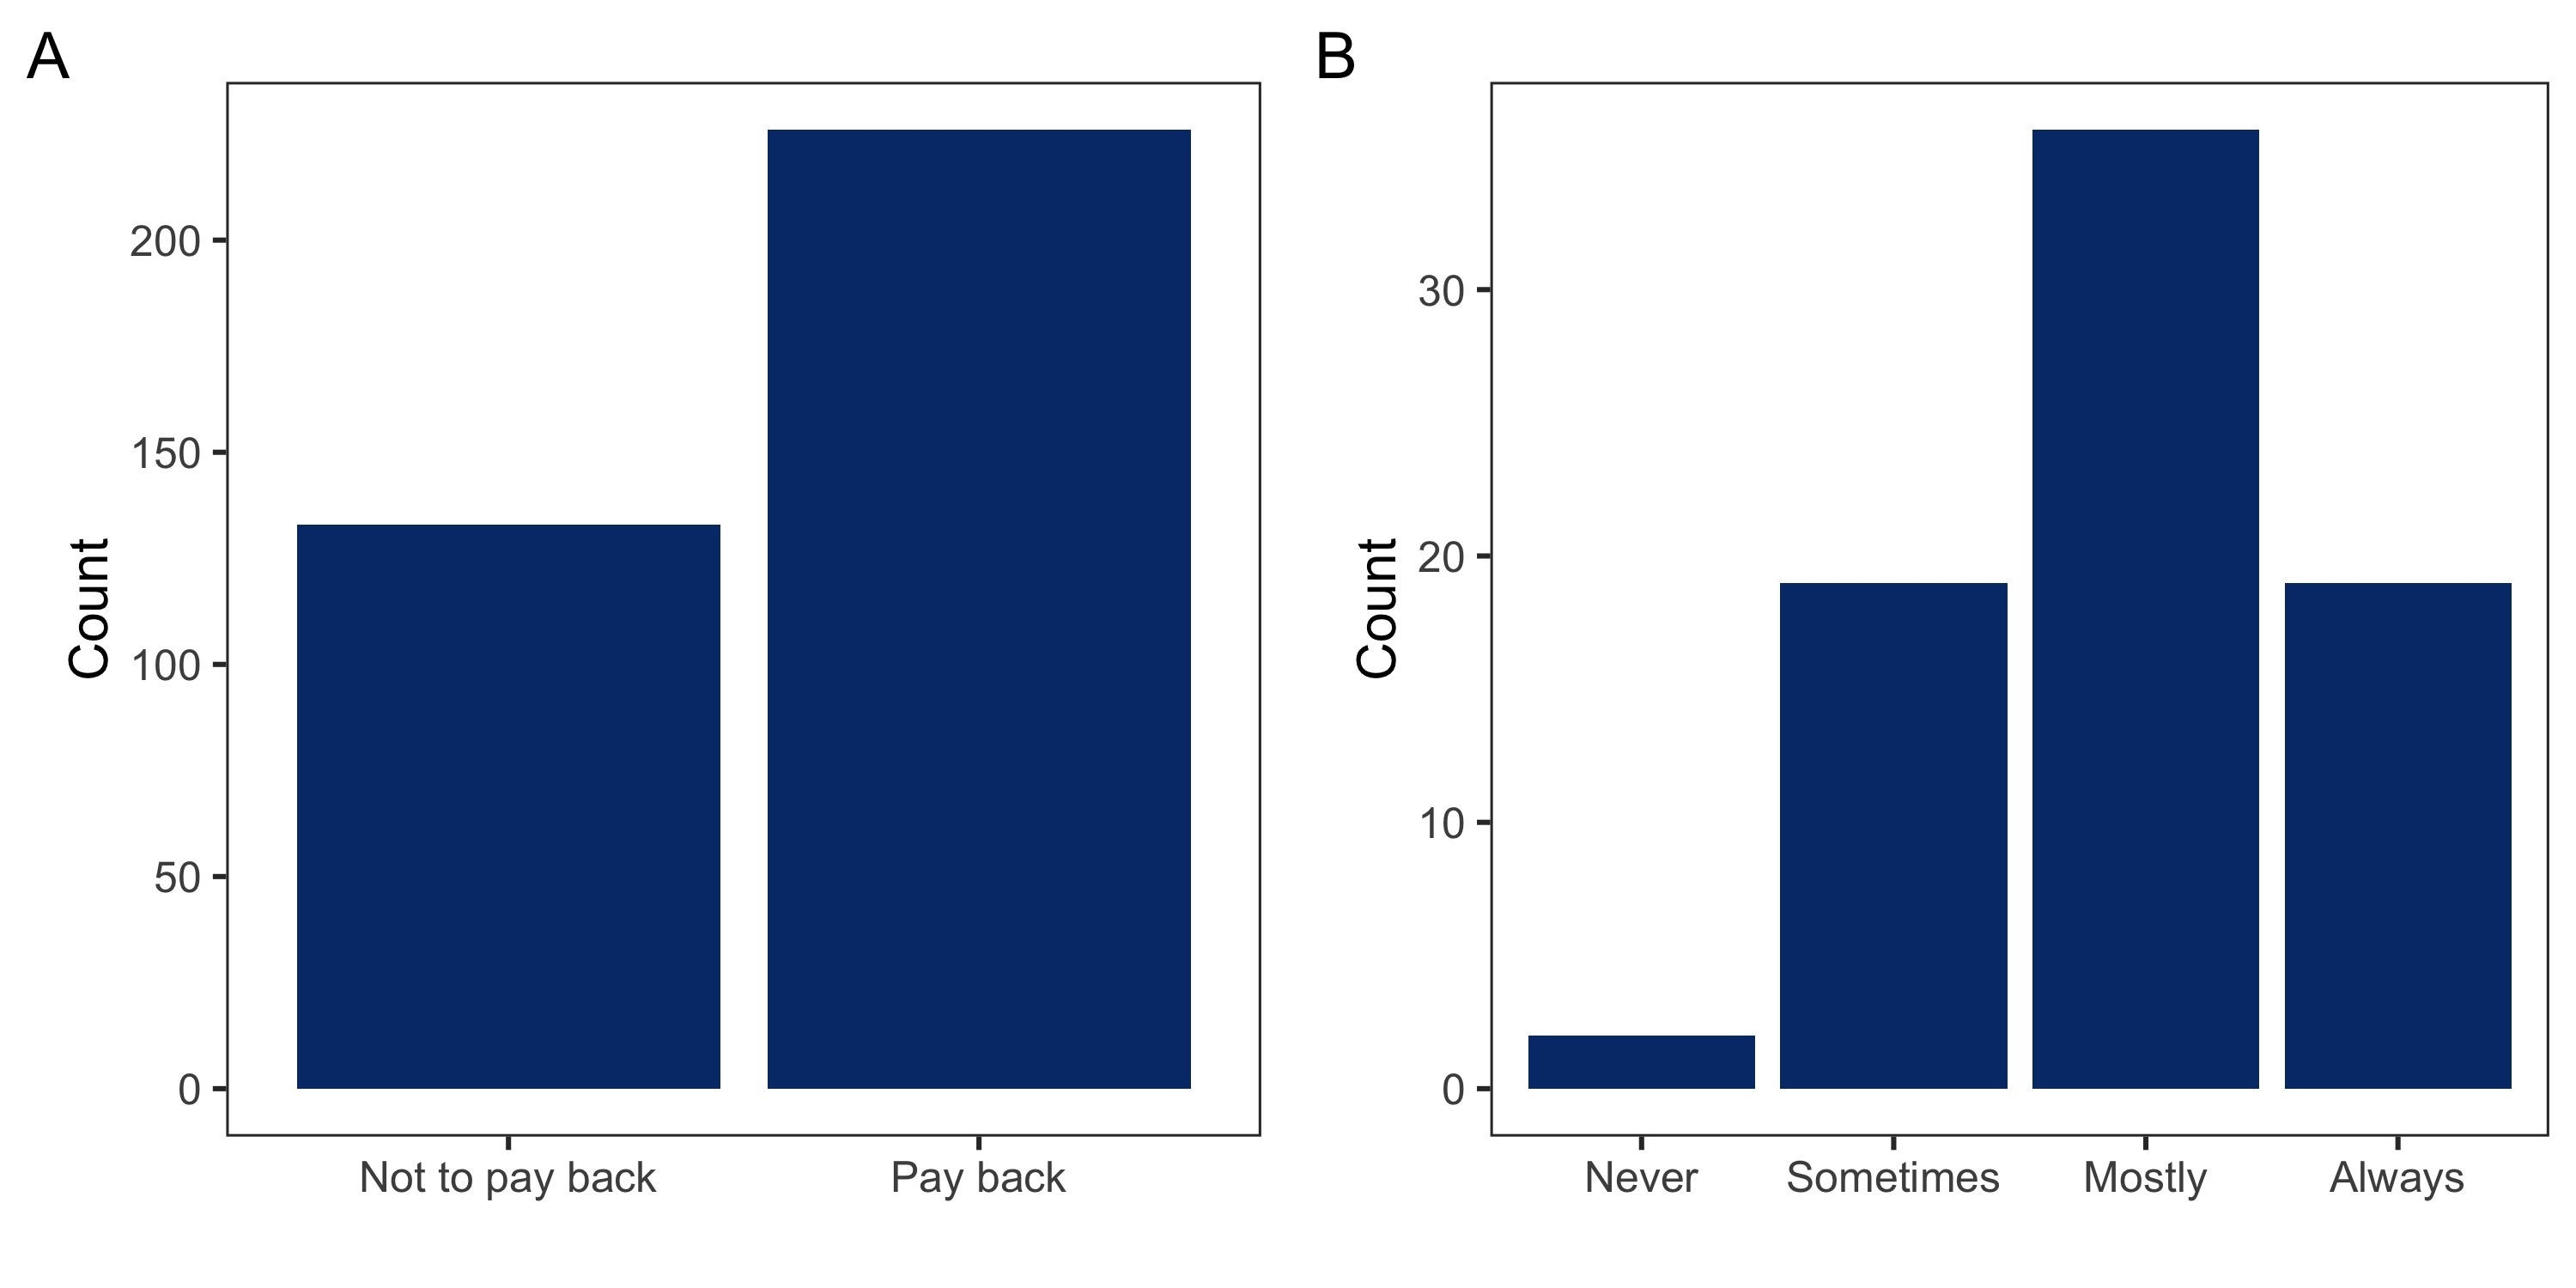
\includegraphics[width=0.8\linewidth]{/Users/saidjimenez/Documents/R/github_Said/social_closeness/Manuscript/figures/fig1} 

}

\caption{Frecuencies of paying and Promise choice}\label{fig:fig2}
\end{figure}

\begin{figure}

{\centering 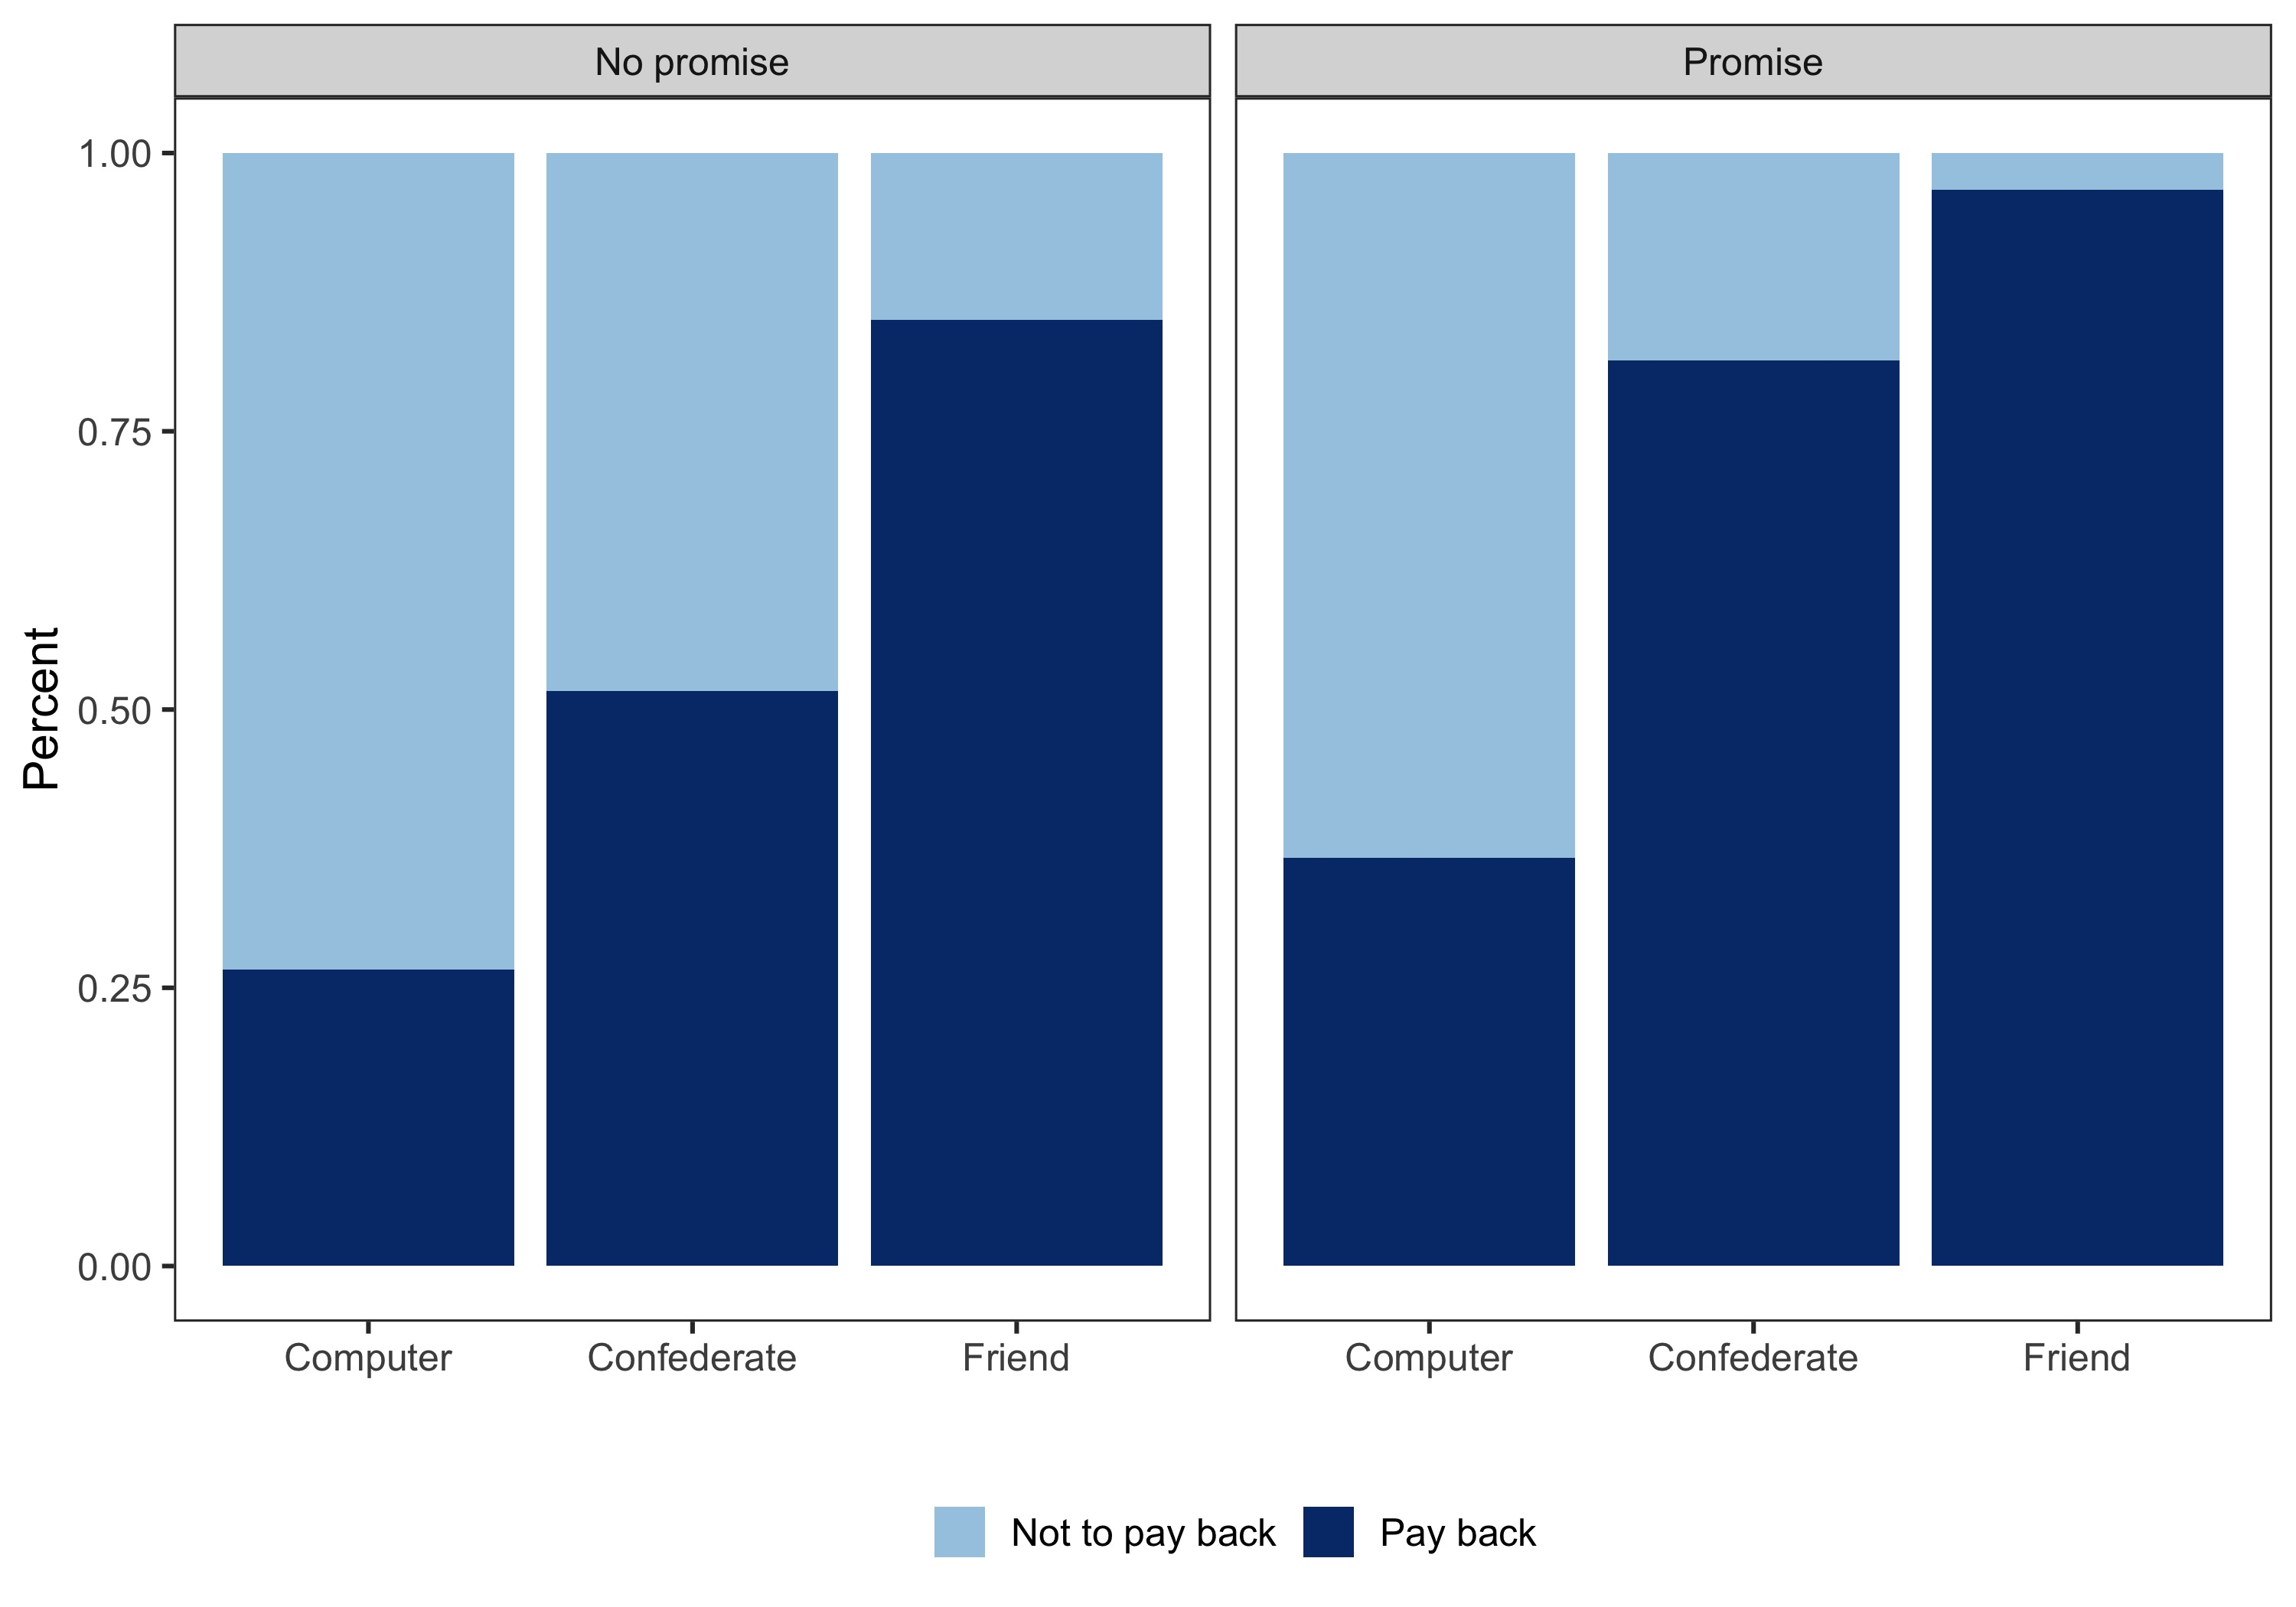
\includegraphics[width=0.8\linewidth]{/Users/saidjimenez/Documents/R/github_Said/social_closeness/Manuscript/figures/fig2} 

}

\caption{Rates by partners and promise condition}\label{fig:fig3}
\end{figure}

\subsubsection{Resultados: modelo
jerárquico}\label{resultados-modelo-jerarquico}

En la tabla 1, se muestran los efectos poblacionales del modelo
bayesiano jerárquico para la tasa de pago. Se presentan las estimaciones
de cada coeficiente del modelo en escala \emph{logit}, su error estándar
y los intervalos de credibilidad bayesianos del 95\%. Los cuales indican
los límites inferiores y superiores de las estimaciones entre los que se
ubica el 95 \% de probabilidad.

Table 1. Population-Level Effects of Task

\begin{longtable}[]{@{}lrrrr@{}}
\toprule
Term & Estimate & SE & L-95\% CI & U-95\% CI\tabularnewline
\midrule
\endhead
\(\beta^0\) & -1.62 & 0.40 & -2.31 & -1.02\tabularnewline
\(\beta^{promise}\) & 1.27 & 0.40 & 0.64 & 1.92\tabularnewline
\(\beta^{confederate}\) & 2.01 & 0.55 & 1.20 & 2.97\tabularnewline
\(\beta^{friend}\) & 4.15 & 0.77 & 3.07 & 5.49\tabularnewline
\bottomrule
\end{longtable}

La figura 4A muestra la incertidumbre con respecto a la estimación de
los coeficientes, la linea central indica la mediana de la distribución
y el área sombreada el intervalo del 50 \% de probabilidad. Se puede
observar que la condición de promesas y cercanía social alta (amigo)
obtuvieron estimaciones mayores que el intercepto, que para este caso
podría considerarse la estimación del efecto de la ausencia de promesas
y cercanía social.

Para visualizar el efecto conjunto de las condiciones experimentales en
la probabilidad de pagar la mitad, se realizó su combinación lineal para
obtener un sólo predictor (\(\mathrm{linpred_i}\)), se le aplicó la
función ligadora inversa \emph{logit} y se transformó su output en
probabilidades por medio de la función logistica
\(1 / (1 + \exp(-\mathrm{linpred}_i))\). La figura 4B muestra la
probabilidad de pagar la mitad, como función de la combinación lineal de
las condiciones experimentales, las lineas delgadas muestran la
incertidumbre en la predicción con una muestra aleatoria de tamaño 100
de las distribuciones posteriores de los parámetros poblacionales. La
linea gruesa representa la media de las distribuciones posteriores de
los parámetros poblacionales. Se puede observar, que a medida que se
incrementa el valor del predictor lineal, se incrementa rápidamente la
probabilidad de pago. Cabe destacar que el el valor del predictor lineal
aumenta con la presencia de las condiciones experimentales de cercanía
social y promesas.

\begin{figure}

{\centering 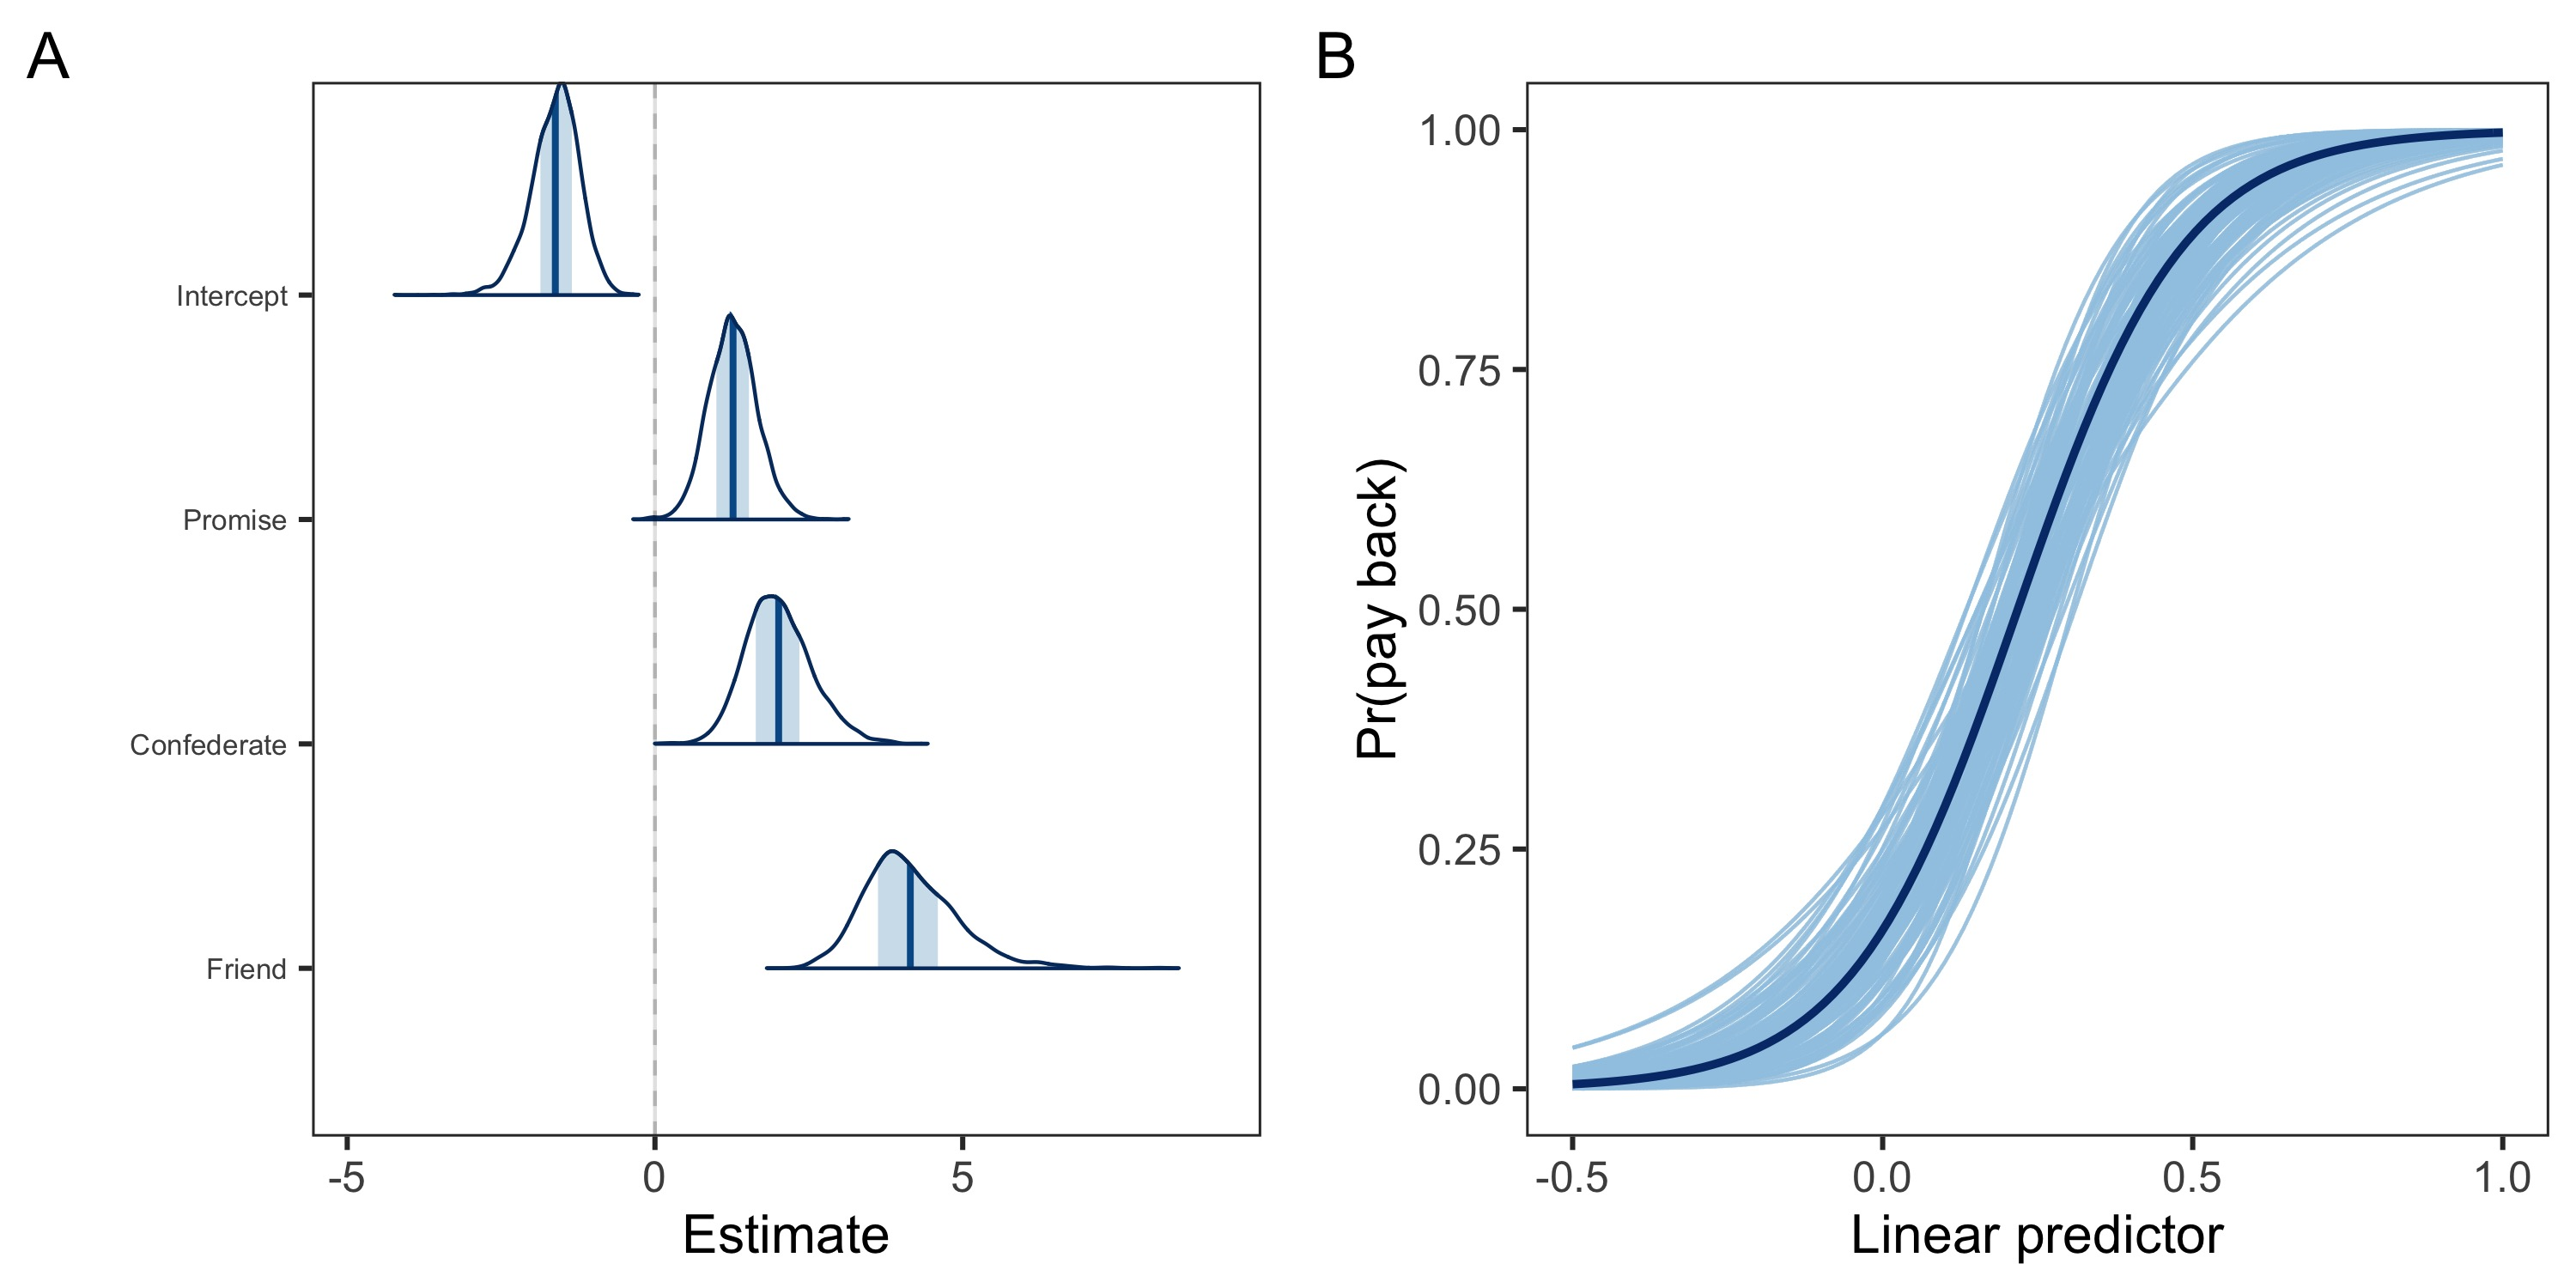
\includegraphics[width=0.8\linewidth]{/Users/saidjimenez/Documents/R/github_Said/social_closeness/Manuscript/figures/fig3} 

}

\caption{Estimates with uncertainty and linear predictor}\label{fig:fig4}
\end{figure}

En un procedimiento similar al descrito para la figura 4B, la figura 5
representa el efecto conjunto de las condiciones experimentales en la
probabilidad de pagar la mitad para cada sujeto. Ya que el modelo
jerárquico asume que las diferencias individuales se pueden modelar
realizando un ajuste \(u\) a los coeficientes poblacionales \(\beta\),
se obtuvieron 50 muestras aleatorias de las distribuciones posteriores
de los parámetros \(u\) para cada sujeto, se realizó el ajuste al modelo
poblacional y se presenta en lineas delgadas la incertidumbre en la
predicción individual.

Se puede observar en algunos sujetos (e.g sujeto 2 ó 17) que a medida
que incrementa el predictor lineal, aumenta rápidamente la probabilidad
de pago, sin embargo, para otros (e.g.~sujeto 1 ó 5), existe
incertidumbre respecto al efecto del predictor lineal, lo que sugiere
que aún en la condición de promesas y en presencia de compañeros con
cercanía social, el participante podría no pagar. La incertidumbre en la
predicción de las respuestas de algunos jugadores, sugiere que podrían
existir por lo menos dos procesos cognitivos que podrían dar lugar las
decisiones observadas, lo que se explora con mayor detenimiento con el
modelo de mezclas latentes.

\begin{figure}

{\centering 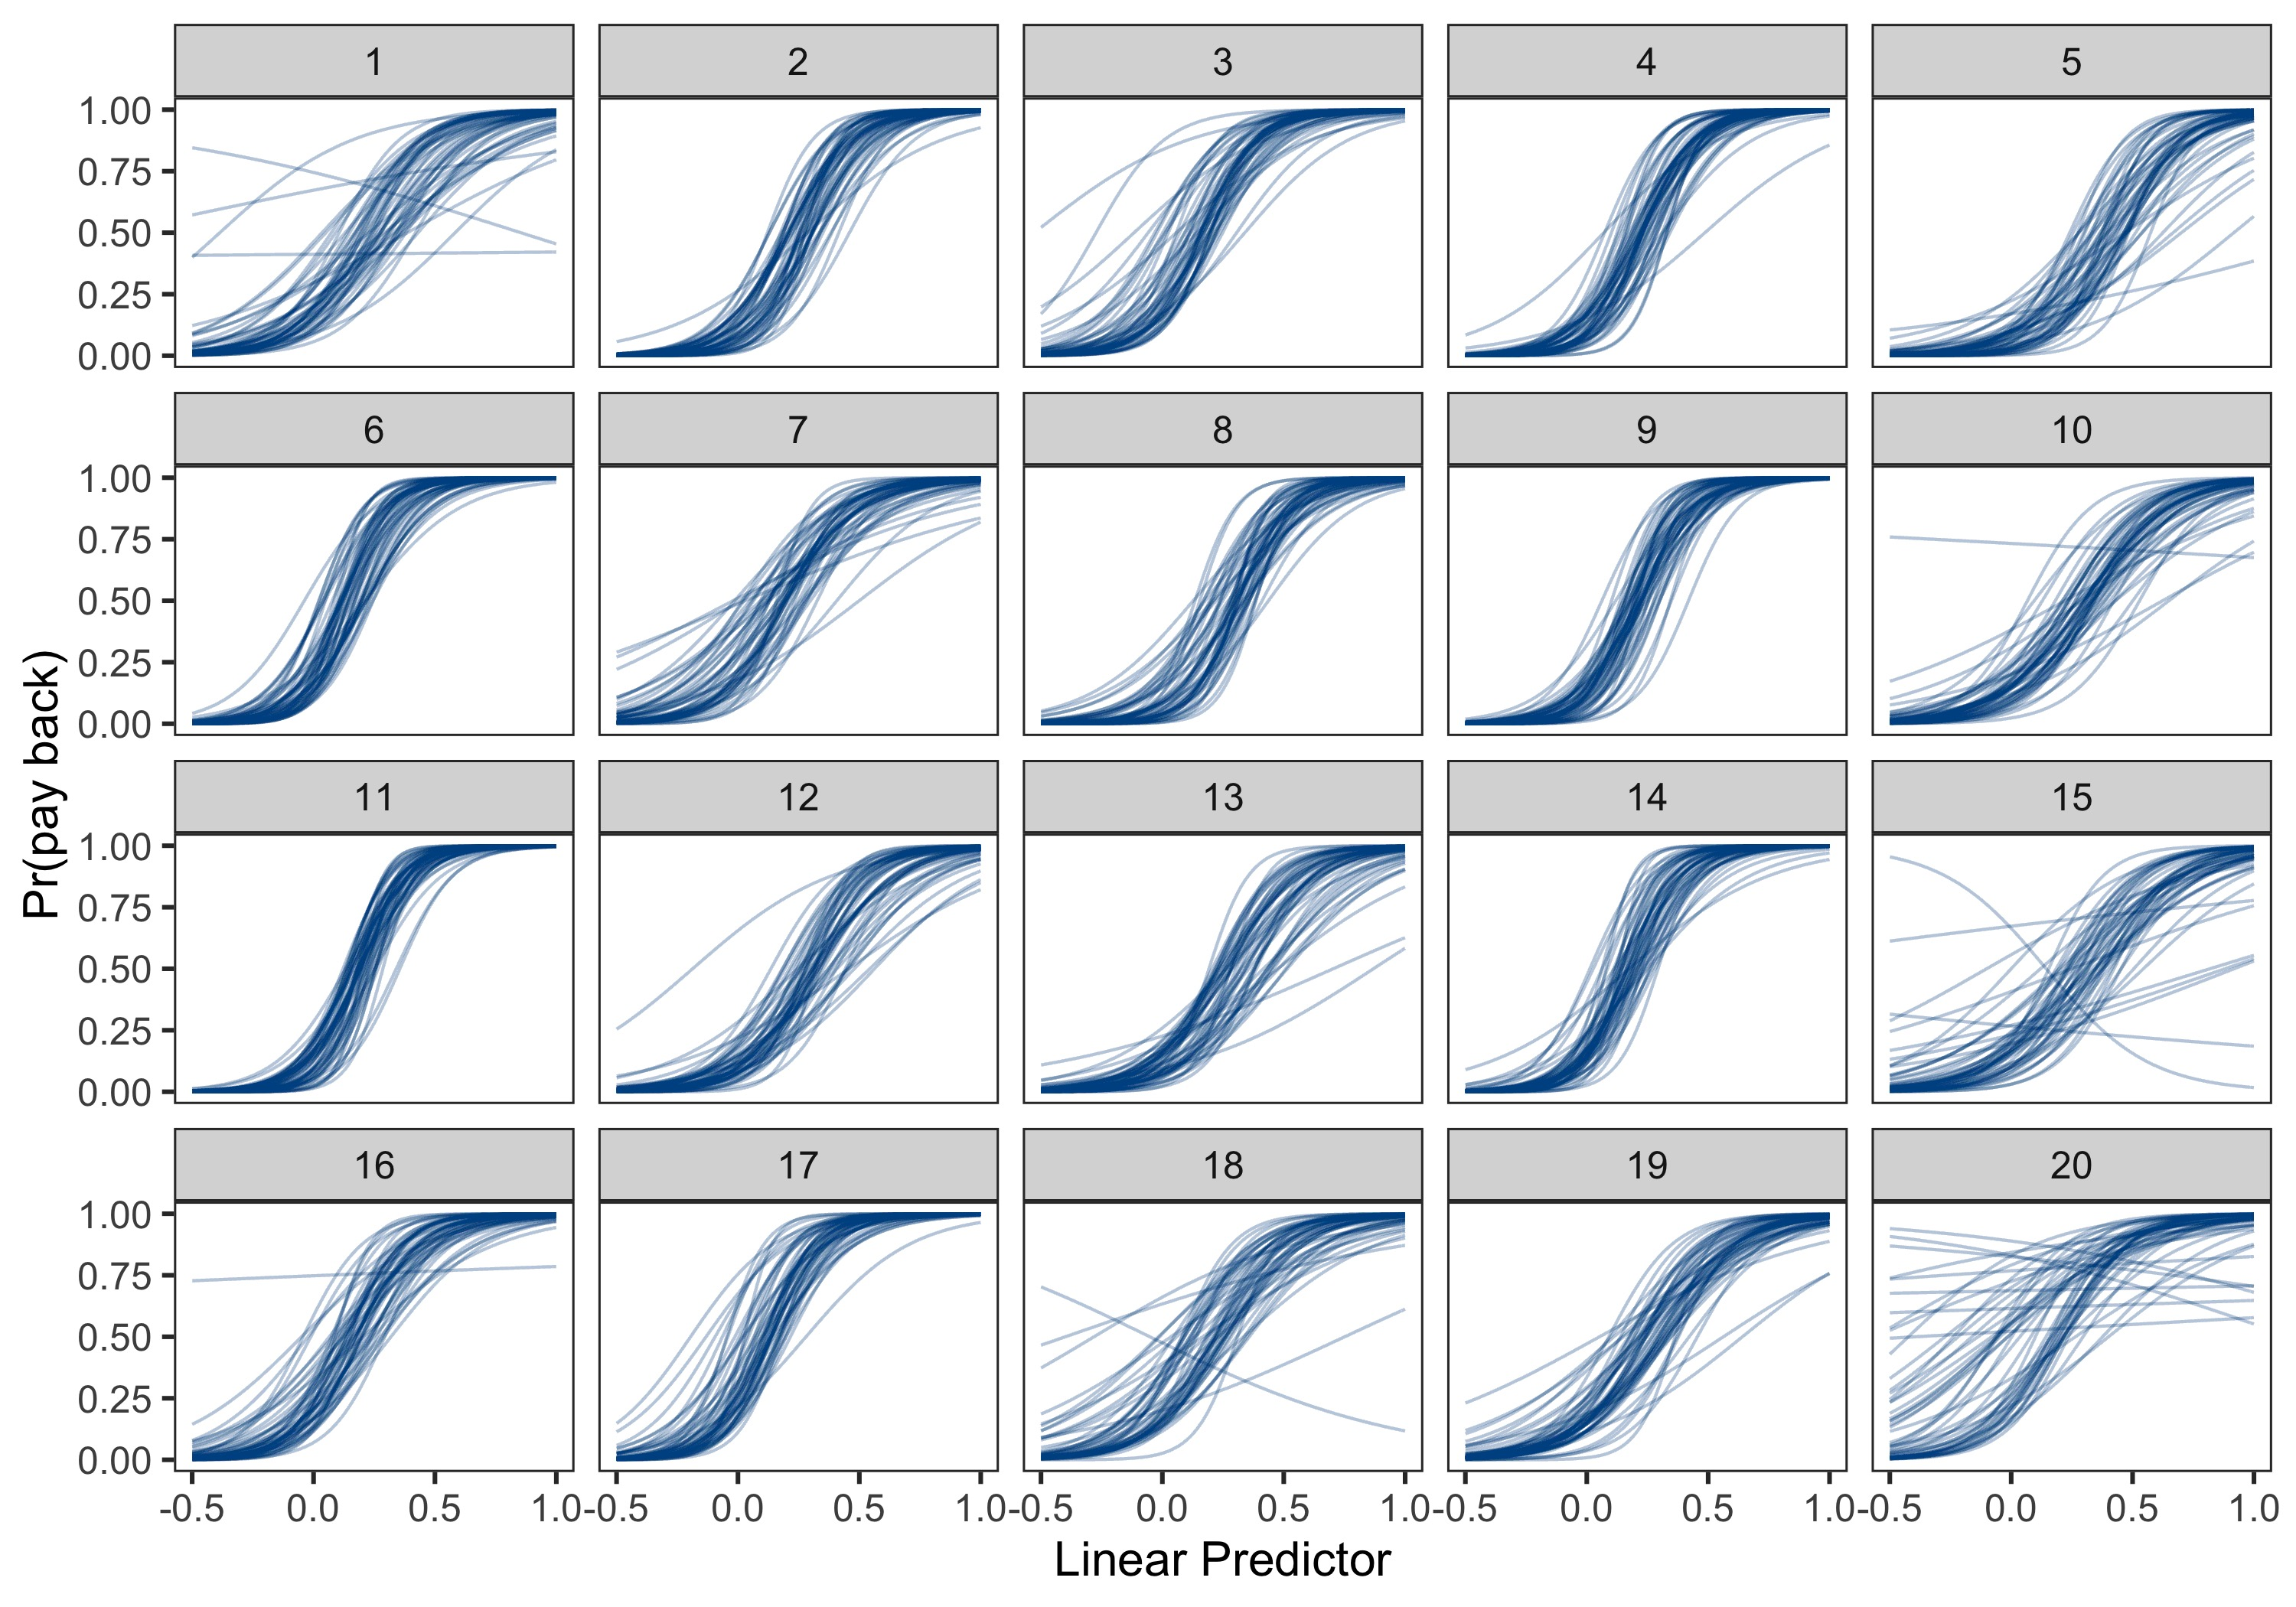
\includegraphics[width=0.8\linewidth]{/Users/saidjimenez/Documents/R/github_Said/social_closeness/Manuscript/figures/g9} 

}

\caption{Estimates with uncertainty by subject}\label{fig:fig5}
\end{figure}

La \textbf{distribución posterior predictiva} consiste en simular el
tipo de observaciones que podrían surgir con el modelo original, pero
una vez que los parámetros de éste han sido actualizados con los datos
observados. En este caso, cuando el modelo ha aprendido de las
decisiones de los sujetos, tiene la capacidad de generar una
\emph{``réplica''} de los datos observados, para cada combinación de los
parámetros obtenidos en la distribución posterior.

En la figura 6, se obtuvieron 50 muestras aleatorias de la distribución
posterior de los parámetros poblacionales \(\beta\) y se simularon 50
datasets con las decisiones que se esperarían dado el valor de esos
parámetros. Se presentan en barras las decisiones realizadas por
nuestros participantes \(y\), mientras que el punto con dispersión
muestra la distribución de los valores esperados en las 50
\emph{replicas} \(y_{rep}\). Se puede observar que el modelo reproduce
con bastante precisión los datos observados, lo cual es un indicador del
adecuado ajuste del modelo.

\begin{figure}

{\centering 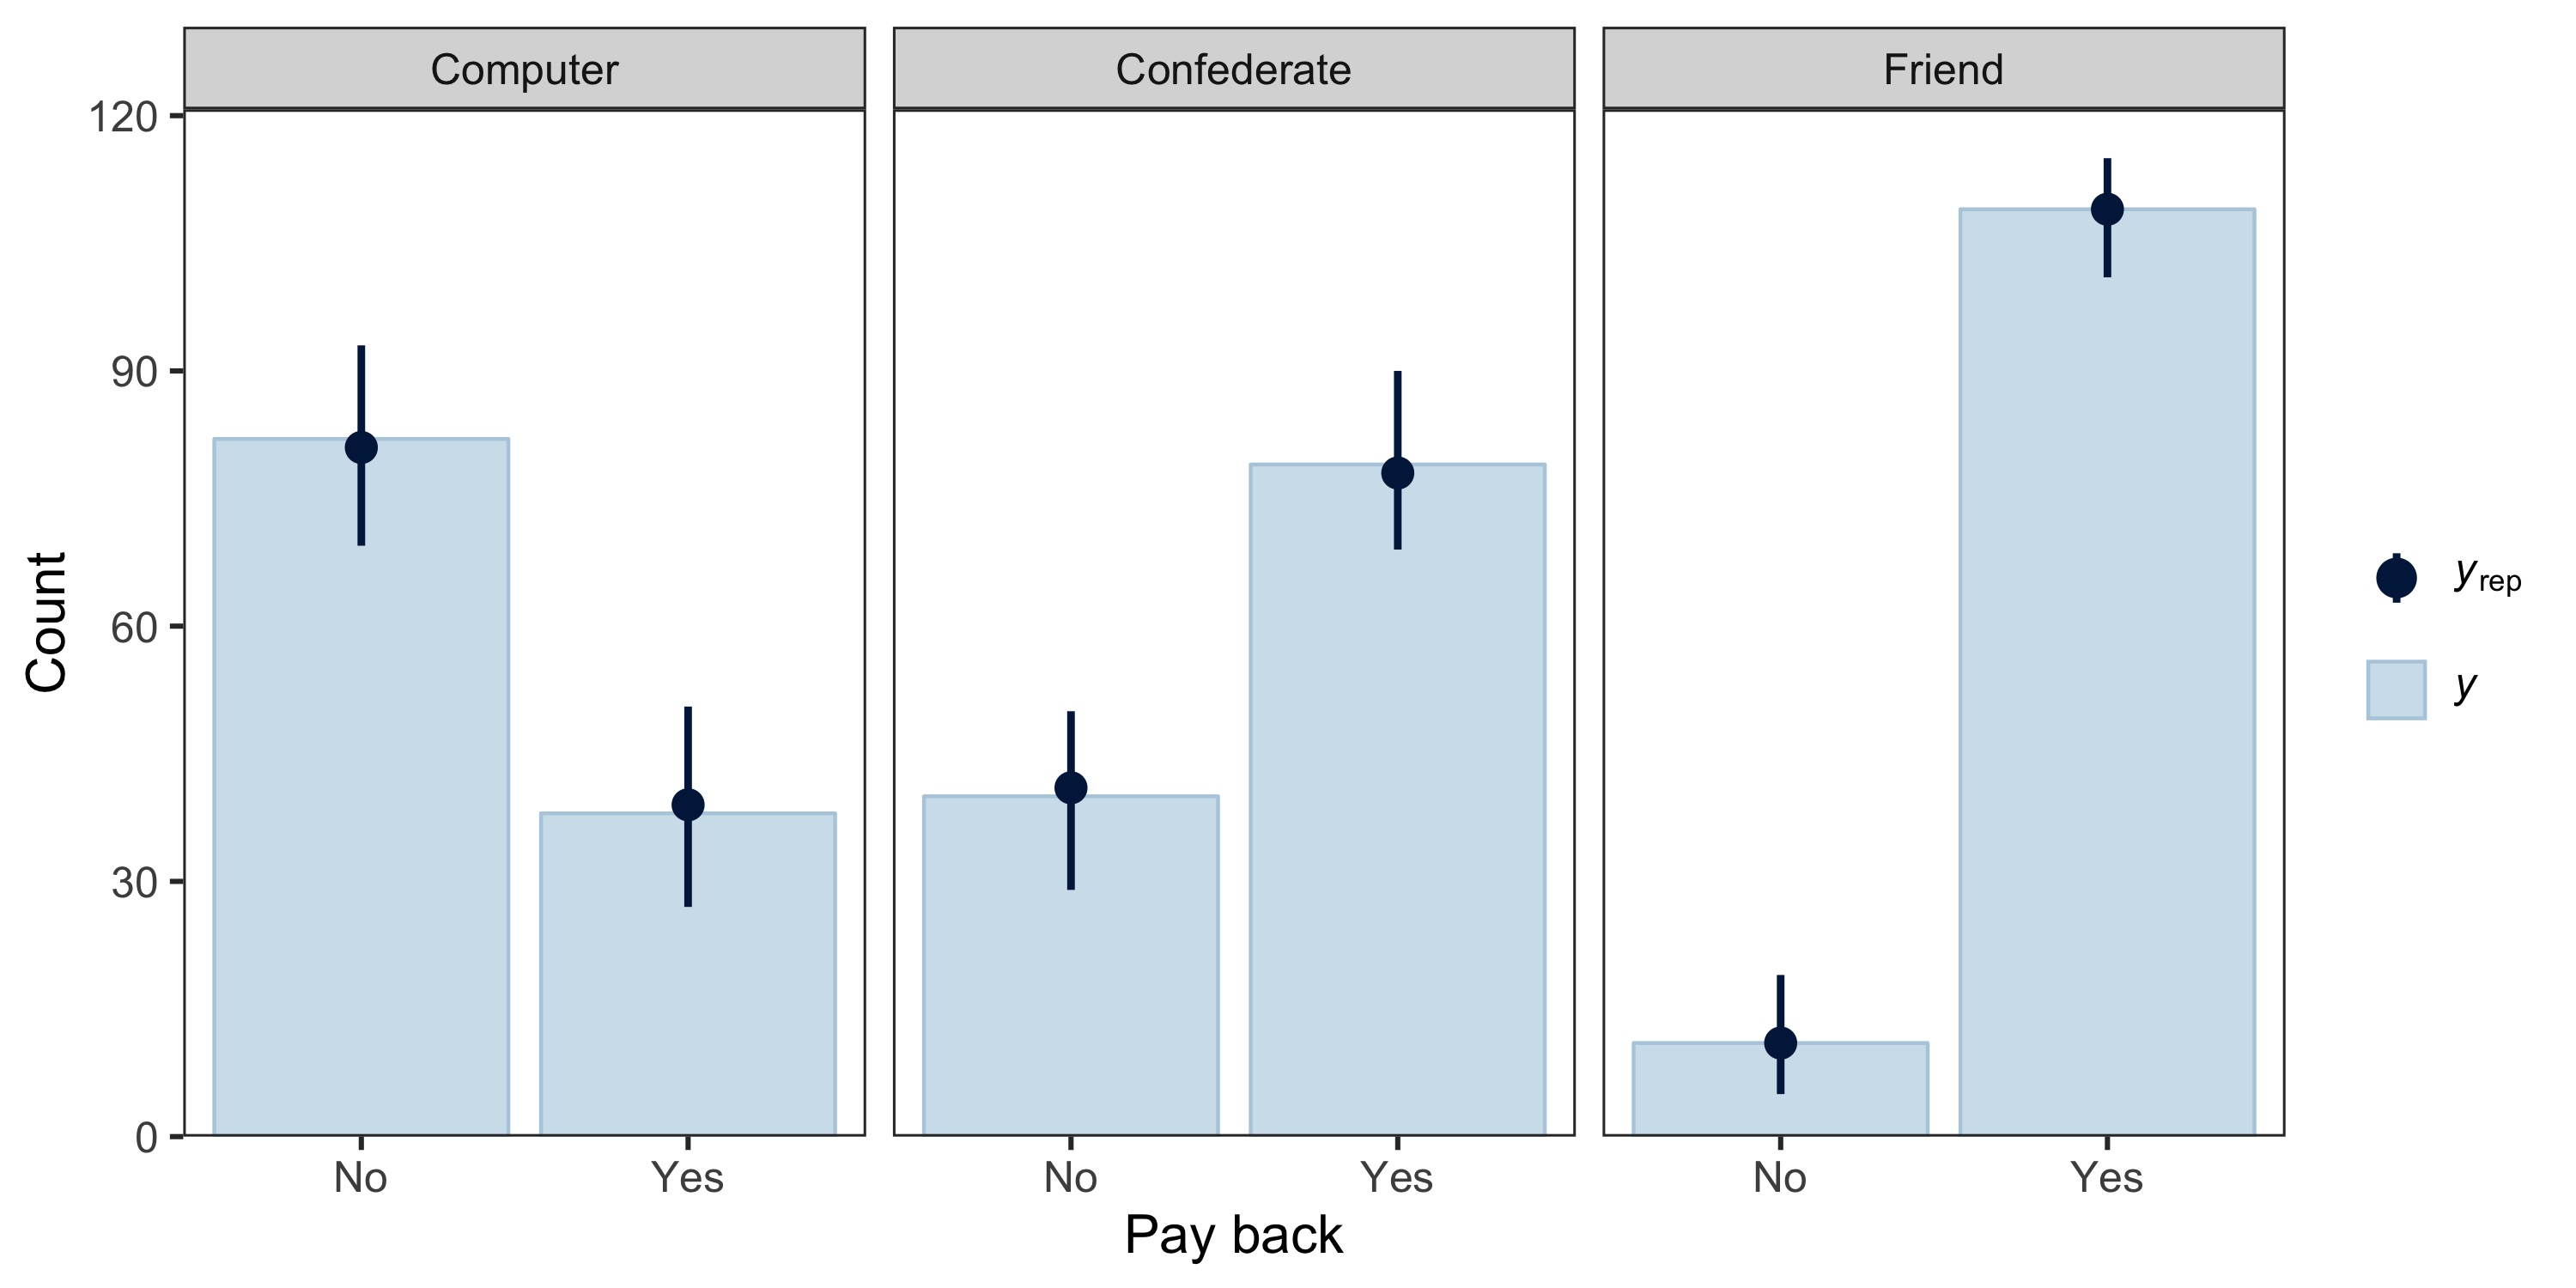
\includegraphics[width=0.8\linewidth]{/Users/saidjimenez/Documents/R/github_Said/social_closeness/Manuscript/figures/fig5} 

}

\caption{Posterior predictive distribution of choices by partner}\label{fig:fig6}
\end{figure}

\subsubsection{Resultados: modelo de mezclas
latentes}\label{resultados-modelo-de-mezclas-latentes}

El modelo de 2-mezclas latentes identificó dos subpoblaciones de tamaño
10; en la tabla 2 se muestran los resúmenes de las distribuciones
posteriores de los parámetros de ambas subpoblaciones y el parámetro de
la mezcla \(\phi\). Una de las subpoblaciones tiene alta probabilidad de
pagar \(\mu_1\), la que denominamos \textbf{honestos} y la otra
subpoblación tiene una probabilidad de pagar menor por lo que fue
denominada \textbf{deshonestos} \(\mu_2\). En la figura 7A se muestran
las distribuciones posteriores de las dos \(\mu\)'s, correspondientes a
la probabilidad de pagar de las dos subpoblaciones latentes. Y en la
figura 7B se presentan las decisiones de dos sujetos extraídos de las
dos subpoblaciones, el sujeto 5 de la subpoblación de
\textbf{deshonestos} y el 17 de la subpoblación de \textbf{honestos}. Se
puede observar que el sujeto 5 decide no pagar en la mayoría de los
ensayos, independientemente de la condición de promesas y cercanía
social, mientras que el sujeto 17 sólo decidió no pagar en tres
ocasiones cuando su compañero fue la computadora.

Table 2. Parameters of 2-Mixture Model

\begin{longtable}[]{@{}lrrrr@{}}
\toprule
Parameter & Mean & SD & L-95\% CI & U-95\% CI\tabularnewline
\midrule
\endhead
\(\mu_{1}\) & 0.56 & 0.05 & 0.44 & 0.65\tabularnewline
\(\mu_{2}\) & 0.70 & 0.05 & 0.61 & 0.82\tabularnewline
\(\lambda_{1}\) & 48.99 & 28.57 & 5.50 & 97.49\tabularnewline
\(\lambda_{2}\) & 54.79 & 26.24 & 7.80 & 97.61\tabularnewline
\(\phi\) & 0.49 & 0.15 & 0.21 & 0.77\tabularnewline
\bottomrule
\end{longtable}

\begin{figure}

{\centering 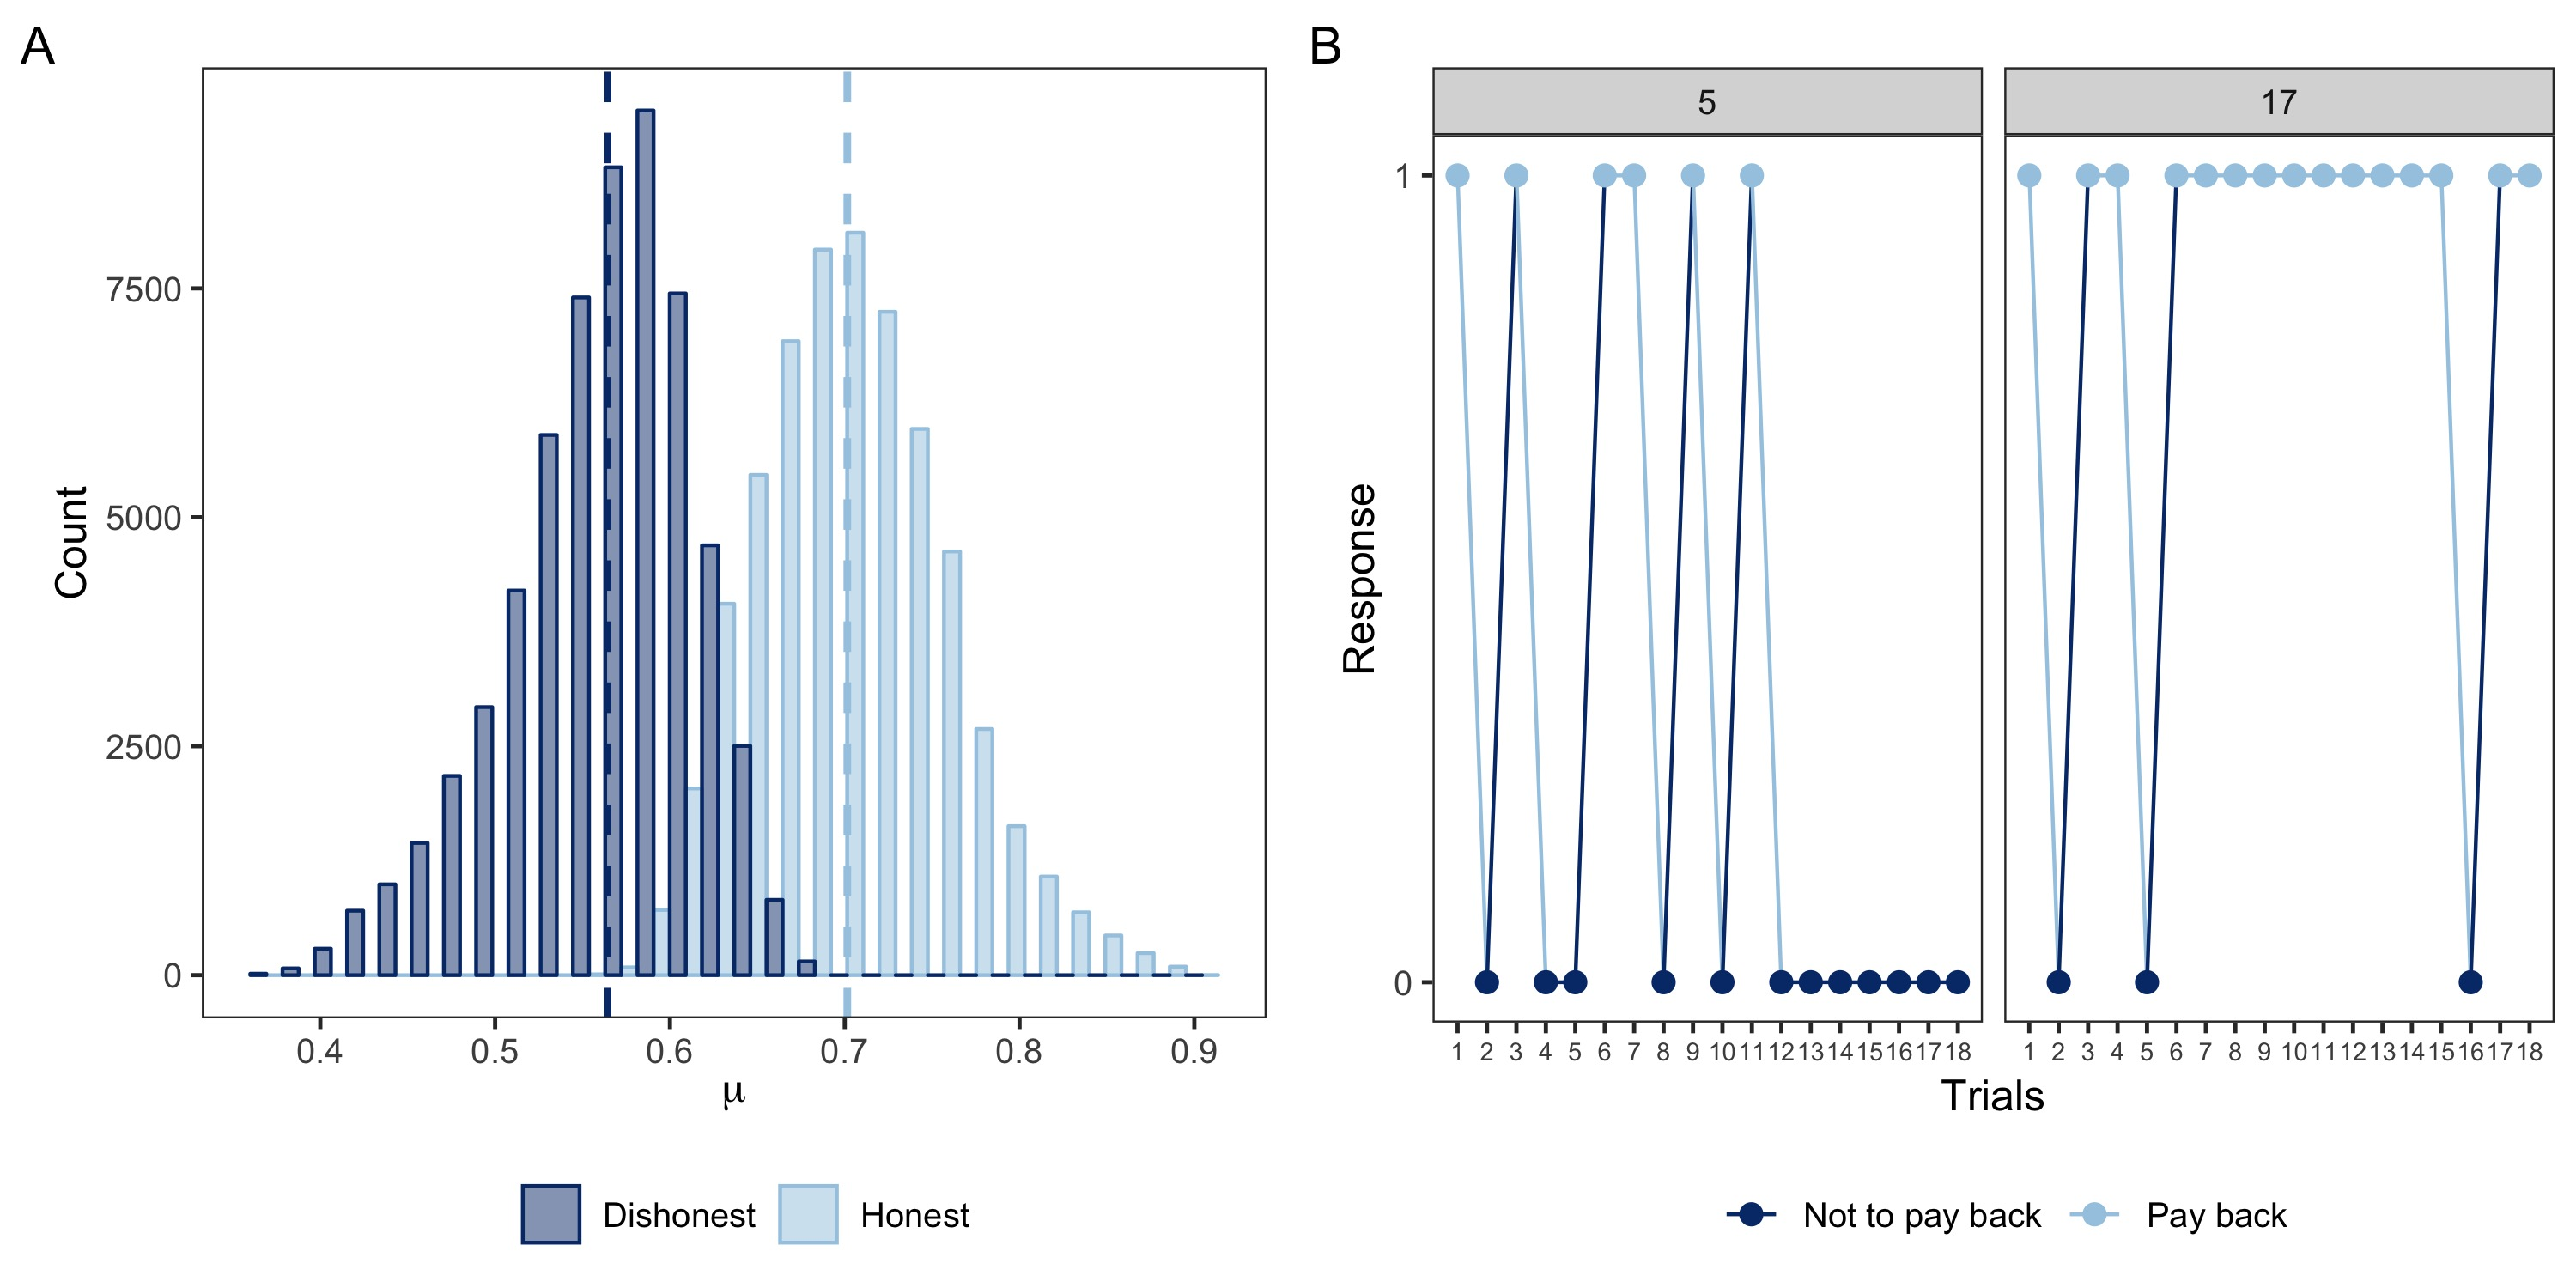
\includegraphics[width=0.8\linewidth]{/Users/saidjimenez/Documents/R/github_Said/social_closeness/Manuscript/figures/fig6} 

}

\caption{Posteriors from two latent groups and two cases}\label{fig:fig7}
\end{figure}

En la figura 8 se muestra la frecuencia de las decisiones de los dos
grupos latentes, dependiendo de si estaban en la condición con o sin
promesa.

\begin{figure}

{\centering 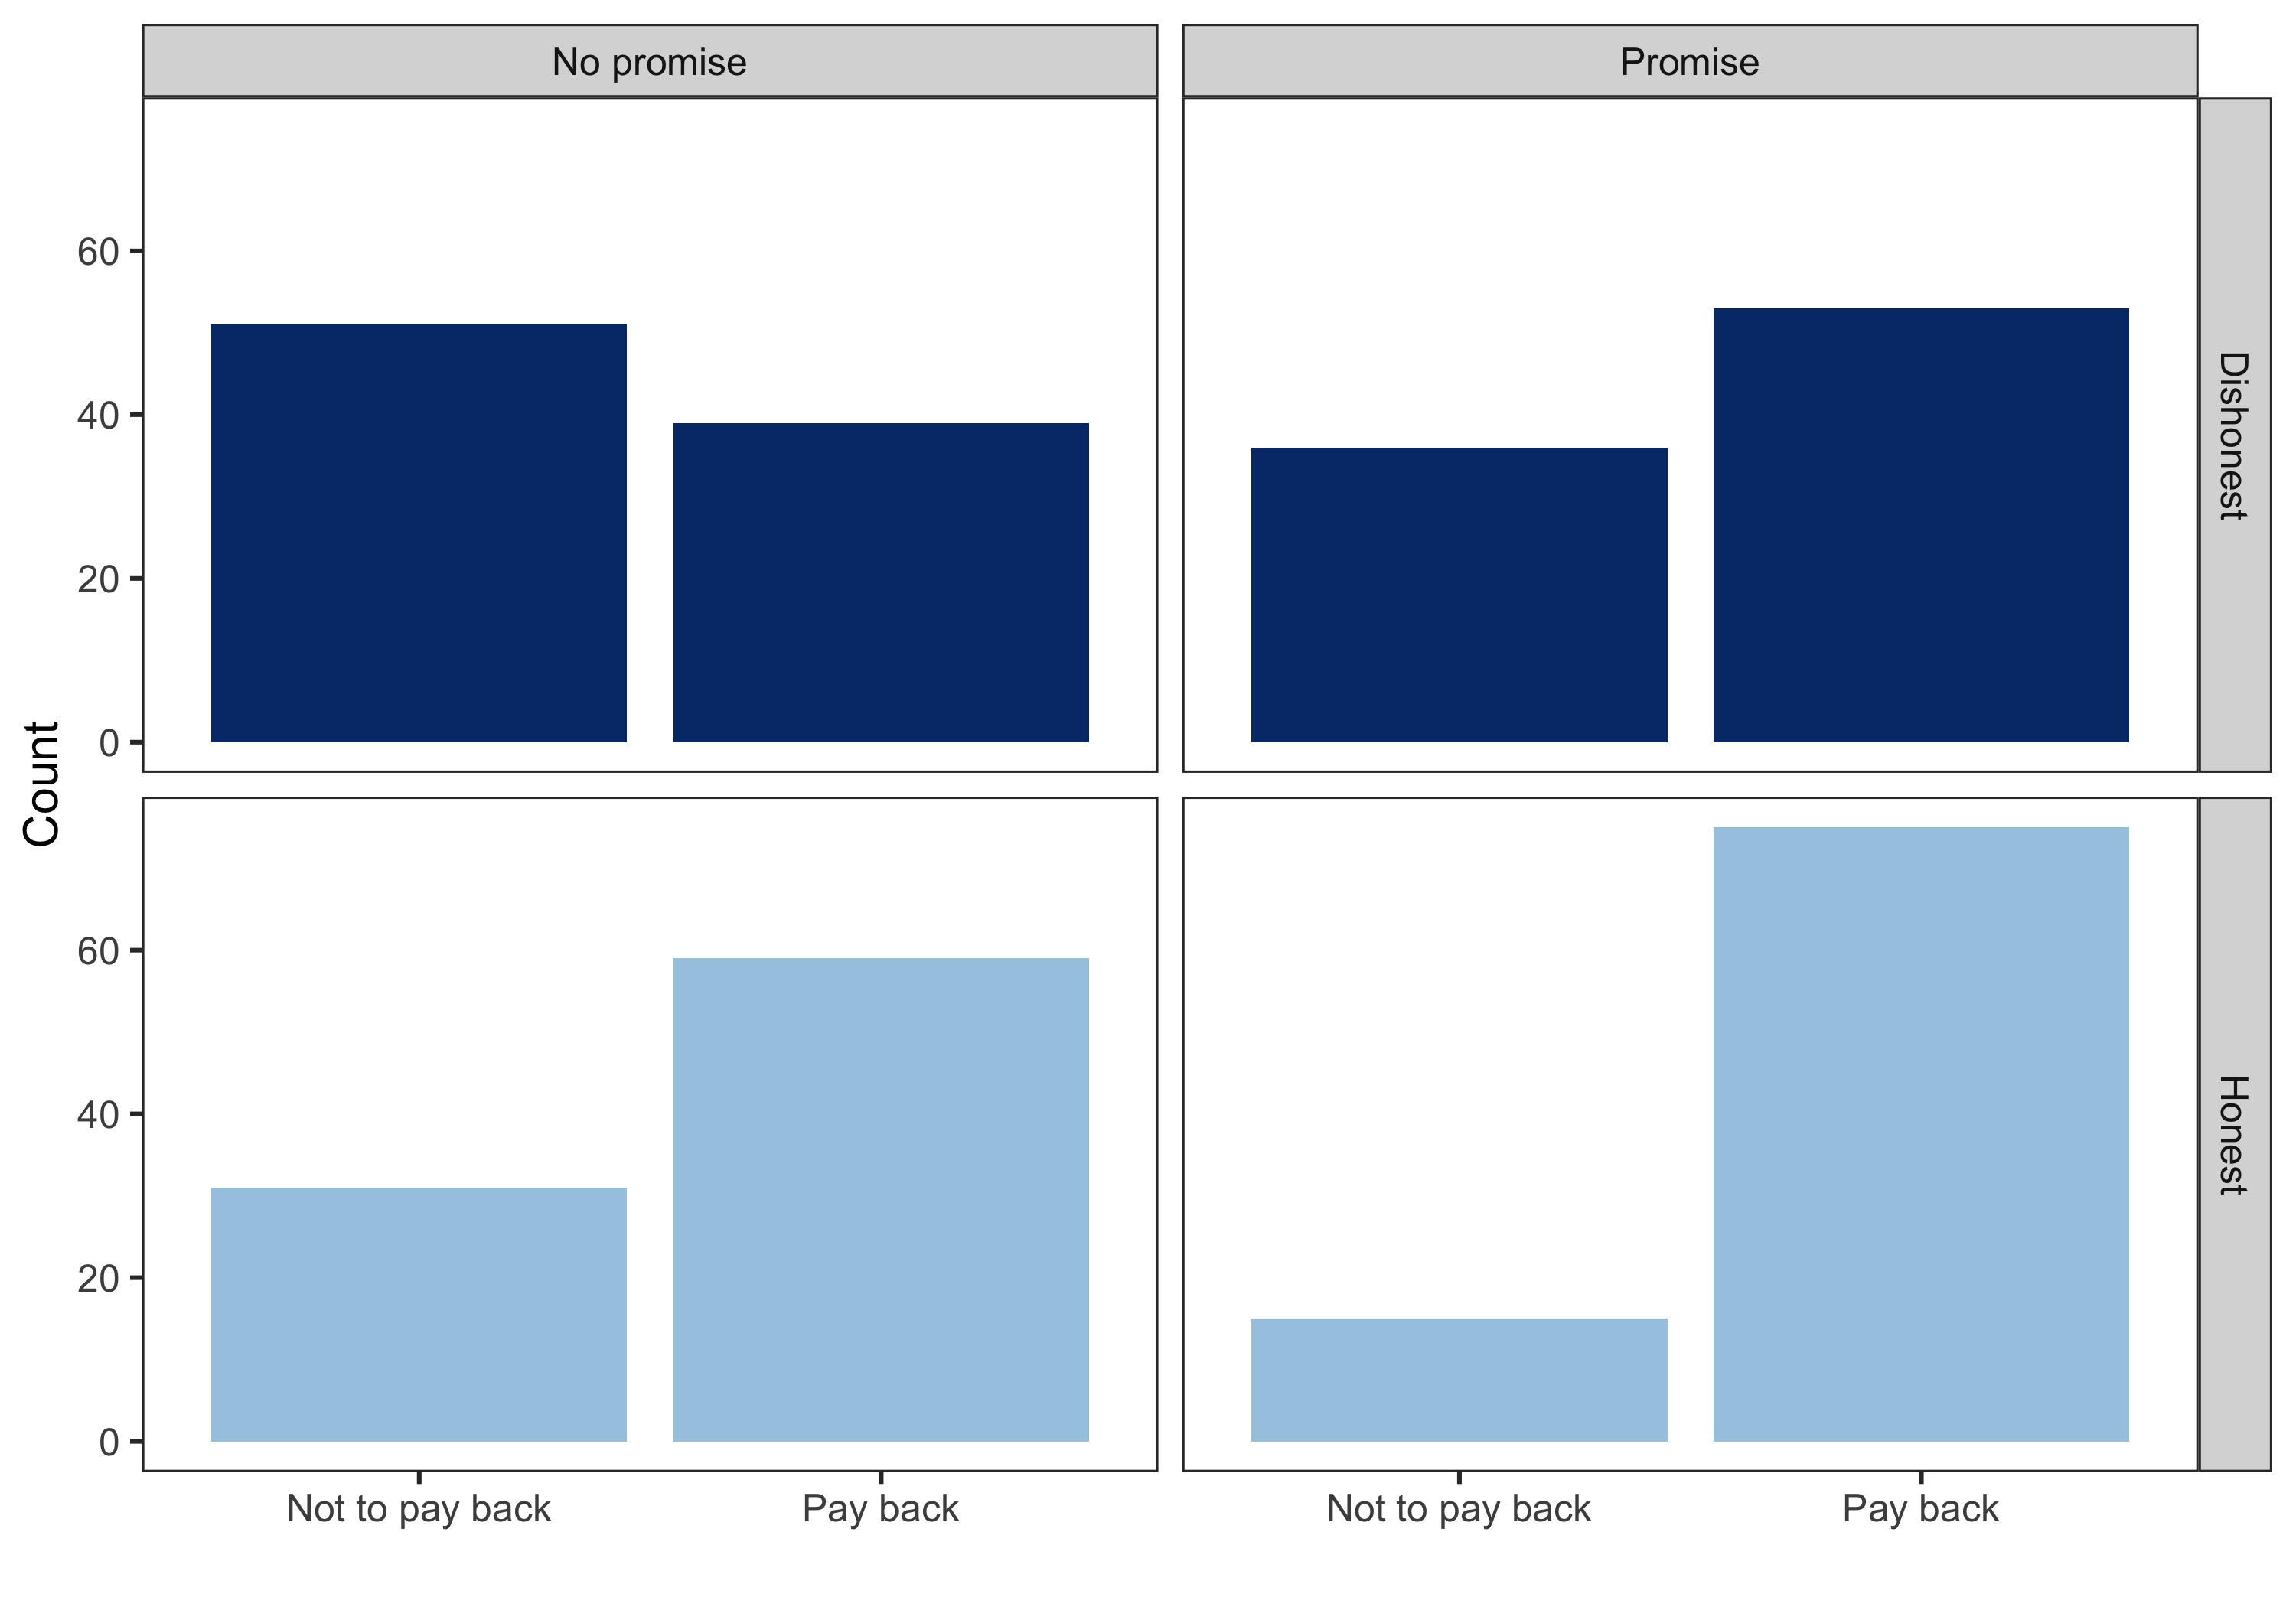
\includegraphics[width=0.8\linewidth]{/Users/saidjimenez/Documents/R/github_Said/social_closeness/Manuscript/figures/g12_b} 

}

\caption{Payment frecuency by latent group and promise condition}\label{fig:fig8}
\end{figure}

\subsubsection{Resultados: tiempo de
reacción}\label{resultados-tiempo-de-reaccion}

En la tabla 3 se presentan las estimaciones poblacionales del modelo
bayesiano de los tiempos de reacción, se resumen las distribuciones
posteriores de cada parámetro, incluyendo la estimación de su media, su
error estándar y los intervalos de credibilidad bayesianos del 95\%. En
la figura 9A se muestran con puntos los tiempos de reacción en segundos
para cada decisión realizada de acuerdo con cada subgrupo, se agregó a
cada grupo un kernel de densidad simétrico para representar la cantidad
de casos acumulados a lo largo de los diferentes valores del tiempo de
reacción.

En la figura 9B se presenta la diferencia de las estimaciones
posteriores, el punto con dispersión representa el estimador puntual de
la diferencia entre las subpoblaciones y el intervalo de credibilidad
bayesiano del 95\%. El histograma representa la distribución posterior
de la diferencia entre los parámetros de las subpoblaciones.

Table 3. Parameters estimates of reaction time model

\begin{longtable}[]{@{}lrrrr@{}}
\toprule
Term & Estimate & SE & L-95\% CI & U-95\% CI\tabularnewline
\midrule
\endhead
\(\mu_{Dishonest}\) & 2.93 & 0.23 & 2.55 & 3.31\tabularnewline
\(\mu_{Honest}\) & 3.06 & 0.22 & 2.69 & 3.42\tabularnewline
\(\mu_{difference}\) & -0.13 & 0.32 & -0.77 & 0.52\tabularnewline
\(\sigma\) & 1.23 & 0.05 & 1.15 & 1.31\tabularnewline
\(\sigma_{subject}\) & 0.65 & 0.14 & 0.45 & 0.89\tabularnewline
\bottomrule
\end{longtable}

\begin{figure}

{\centering 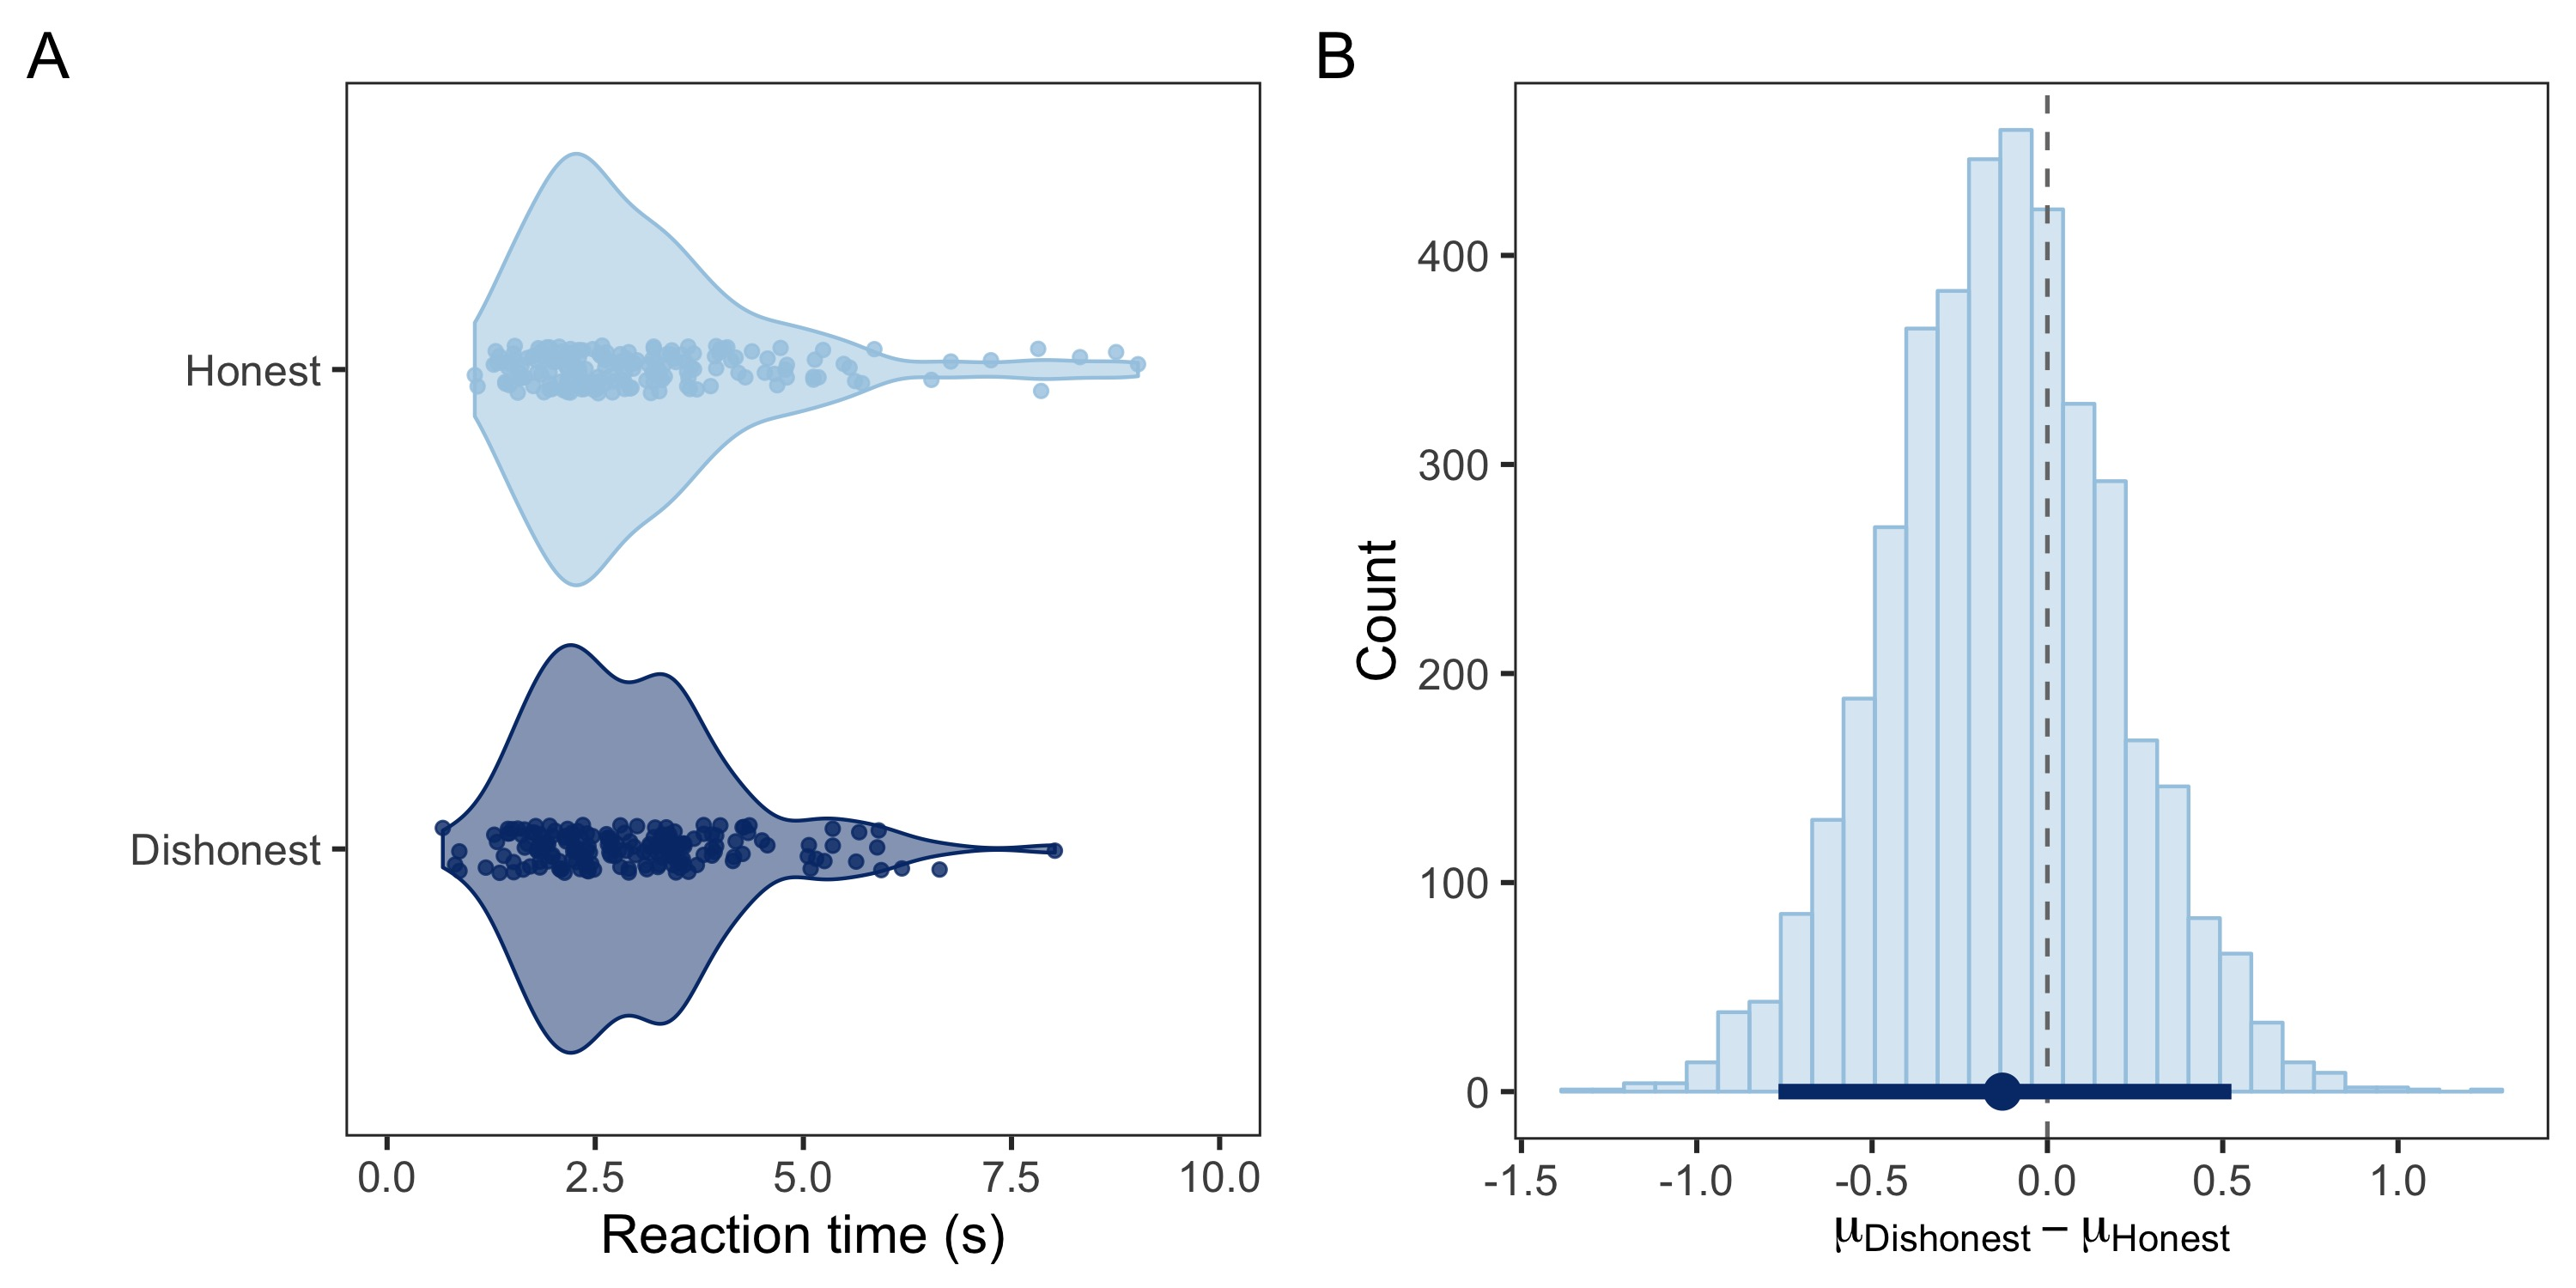
\includegraphics[width=0.8\linewidth]{/Users/saidjimenez/Documents/R/github_Said/social_closeness/Manuscript/figures/fig8} 

}

\caption{Differences in reaction time by latent group}\label{fig:fig9}
\end{figure}

\subsubsection{Resultados: contraste de hipótesis y comparación de
modelos}\label{resultados-contraste-de-hipotesis-y-comparacion-de-modelos}

En la tabla 4 se muestran las hipótesis contrastadas, las estimaciones,
los errores estándar y el factor de Bayes (BF) para cada una. Se
interpretan los BF's como evidencia en favor de la hipótesis alterna
\(BF_{10}\) de acuerdo a la clasificación de Jeffreys (1961). La
hipótesis uno de si la condición de promesas tiene un efecto superior a
0, se interpreta como ``evidencia extrema'' a su favor, la hipótesis de
si el efecto en la tasa de pago es superior para el amigo que para el
confederado también se interpreta como ``evidencia superior'' a su
favor, la hipótesis sobre si la diferencia entre los tiempos de reacción
entre honestos y deshonestos es menor a cero, se interpreta como
``evidencia anecdótica'' a su favor.

Dado que el intervalo de credibilidad bayesiano para la estimación de la
diferencia entre los tiempos de reacción de las subpoblaciones incluye
el cero, se decidió evaluar la hipótesis de si la diferencia es igual a
0, el BF correspondiente se interpreta como ``evidencia fuerte'' en
favor a la diferencia igual a 0. Finalmente, se comparó el DIC para los
modelos de una (\(DIC_{1}\)) y dos (\(DIC_{2}\)) mezclas, cuya
diferencia apoya al modelo de dos mezclas latentes.

Table 4. Hypothesis testing and model comparison

\begin{longtable}[]{@{}lrrr@{}}
\toprule
Hypothesis & Estimate & SE & BF\(_{10}\)\tabularnewline
\midrule
\endhead
\(\beta^{promise} > 0\) & 1.27 & 0.40 & 499\tabularnewline
\(\beta^{friend} - \beta^{confederate} > 0\) & 2.14 & 0.77 &
665.67\tabularnewline
\(\mu_{Dishonest} - \mu_{Honest} < 0\) & -0.13 & 0.32 &
1.96\tabularnewline
\(\mu_{Dishonest} - \mu_{Honest} = 0\) & -0.13 & 0.32 &
20.36\tabularnewline
\(DIC_{1} - DIC_{2}\) & 1.21 & 3.49 & -\tabularnewline
\bottomrule
\end{longtable}


\end{document}
